\section{Architectural Design}
\subsection{Overview}
\subsubsection{System View}
The BBP system employs a hybrid architectural paradigm, primarily structured around a \textbf{3-tier client-server framework}, enhanced by a dedicated \textbf{event-driven architecture} layer. This architecture is the perfect balance for addressing the dual requirements of the system: strict transactional user-facing operations and highly responsive asynchronous background processes.

The 3-tier client-server architecture is the fundamental backbone of the BBP system, providing a clear separation between presentation, application logic and data management. This primary structure is used for the synchronous core functionalities made available by the platform, such as account management, bike path browsing, trip planning and history visualization. While the base 3-tier architecture excels at synchronous request-response tasks, some specific functionalities, such as automatic trip tracking, report generation and user notifications, require a more sophisticated asynchronous implementation. These functionalities are handled by the event-driven layer, implemented inside the application layer, which uses asynchronous messaging patterns to decouple the event producing components from their consumers, in order to make the system fast and available to all users. 

\begin{figure}[H]
    \centering
    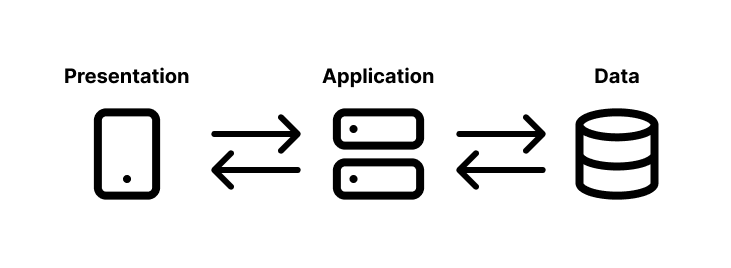
\includegraphics[width=0.5\linewidth]{DD/source/images/diagrams/High Level System View.png}
    \caption{High Level System View. The Event-Driven Layer resides in the Application Layer.}
    \label{fig:high_level_system_view}
\end{figure}

\vspace{0.5cm}\noindent
The adoption of the 3-tier client-server architecture offers several key advantages:
\begin{itemize}
    \item Modular separation of concerns: by decoupling the presentation layer from the back-end logic, the system reduces component coupling. This facilitates parallel development streams and simplifies future maintenance.
    \item Centralized Security: authentication, authorization, session-handling and GDPR-related policies are enforced at the application server level, ensuring consistent and controlled access to sensitive data.
    \item Improved data consistency: a centralized data tier simplifies the management of transactional operations and integrity constraints, which is essential for functionalities such as trip history management, deletion of past trips, and performance statistics computation.
    \item Scalability and performance control: the application tier can be scaled independently of the client and data tiers, allowing the system to handle increased loads caused by browsing, filtering, and ranking operations without excessive architectural complexity.
    \item Controlled integration with external services: interactions with external map and weather services are mediated by the application server, enabling timeout handling, fallback strategies, and graceful degradation in case of service unavailability.
\end{itemize}

\subsubsection{Detailed View}
\paragraph{Presentation Tier} Users interact with the BBP platform via a mobile application, which constitutes the presentation layer of the system. The client is responsible for rendering the user interface, collecting input data from the user and issuing HTTPS requests to the back-end. The presentation layer does not implement any business rule, as it is only responsible for displaying information collected from the application layer, collecting sensor data and GPS data and triggering actions such as registration, login, browsing, trip planning, report validation and configuration of preferences.

\paragraph{Application Tier}
The application layer hosts the core services of the BBP system and it's responsible for coordinating all the interactions between each internal service it is composed of, but also between the system and the external services. This layer exposes a set of APIs consumed by the client and it's responsible for enforcing security and privacy constraints, such as authentication, authorization, GDPR-related consent handling, retention rules and secure password storage. From a more practical perspective, the application tier has a micro-service structure, where each component is responsible for a single service:
\begin{itemize}
    \item Account Management: responsible for registration, login, profile updates, account deletion and user preferences management.
    \item Bike Path Inventory: responsible for browsing, filtering and getting path data like scores and obstacles.
    \item Trip Management: responsible for retrieving planned trips, completed trips, but also for the deletion of past trips and the computation of statistics.
    \item Reporting Management: responsible for manual report creation, automatic report generation, user review, validation and publication.
    \item Context Enrichment: responsible for the integration of the external weather service and map service, when required.
\end{itemize}
The application tier also acts as the controlled integration point for the external services, applying timeout handling, input/output validation, and graceful degradation when a provider is unavailable.

The system, as already mentioned, primarily relies on synchronous request-response interactions to support user operations such as authentication, profile management, bike path browsing and trip planning. In this model, each request is handled within a single execution flow, allowing the system to provide immediate feedback to the user. While this approach is well suited for interactive functionalities, it becomes inadequate when applied to operations characterized by continuous data generation, variable computation cost or dependence on external systems. In a purely synchronous implementation, functionalities such as automatic trip tracking, automatic report generation, and trip alert evaluation would require the application server to process data immediately at the moment it is received. This would introduce several issues, including unnecessary resource consumption, increased coupling between system components, and a direct impact on the performance of user-facing services. To overcome these limitations, the application tier integrates an event-driven layer that enables selected functionalities to be handled asynchronously. Instead of forcing immediate processing, relevant domain occurrences are modelled as events and published to an event bus, where they can be buffered and processed by dedicated consumers independently from synchronous user 
interactions. In the BBP system, this architectural choice is motivated by the following considerations:
\begin{itemize}
    \item Trip Alerts: in a synchronous design, the system would need to continuously poll external weather services or repeatedly check obstacle updates in order to detect relevant changes, resulting in unnecessary resource usage and delayed notifications. By adopting an event-driven approach, alerts are triggered only when significant updates occur, allowing the system to react without restoring to inefficient polling mechanisms.
    \item Automatic trip tracking ingestion and processing: tracking data generated by the user's device may be produced at high and variable frequencies. Processing each data fragment synchronously at the time of generation would directly compete with other user-facing operations, such as browsing or trip planning. Through the event-driven layer, tracking data is published as events and temporarily buffered, enabling the system to decouple data ingestion from processing and to absorb peaks in data production without affecting overall responsiveness.
    \item Automatic report generation workflow: generating an automatic trip report may require aggregating a variable amount of tracking data and performing non-trivial computations. If implemented synchronously at the exact moment a trip ends, this process would slow down the handling of other concurrent requests. By triggering report generation asynchronously, the system can produce the report progressively in background, controlling computational load and ensuring that synchronous services remain responsive.
\end{itemize}

By decoupling data production from data processing, the event-driven layer improves scalability, fault tolerance through buffering and retries, and system responsiveness, while preserving the overall 3-tier client–server architecture of the BBP system.

\paragraph{Data Tier}
The data layer is responsible for persistent storage and retrieval of all system data, including user accounts and profile data, consent and tracking preferences, bike paths inventory, planned and completed trips, reports (manual and automatic), and derived statistics. Access to the data tier is mediated exclusively by the application tier, ensuring consistent enforcement of business rules and privacy constraints. 

The centralized data tier simplifies consistency requirements, such as ensuring that deleted trips do not appear in history views or aggregated statistics. It also supports reliability through standard mechanisms (e.g., backup, replication strategies, and indexing), while remaining isolated from direct client access.

\begin{figure}[H]
    \centering
    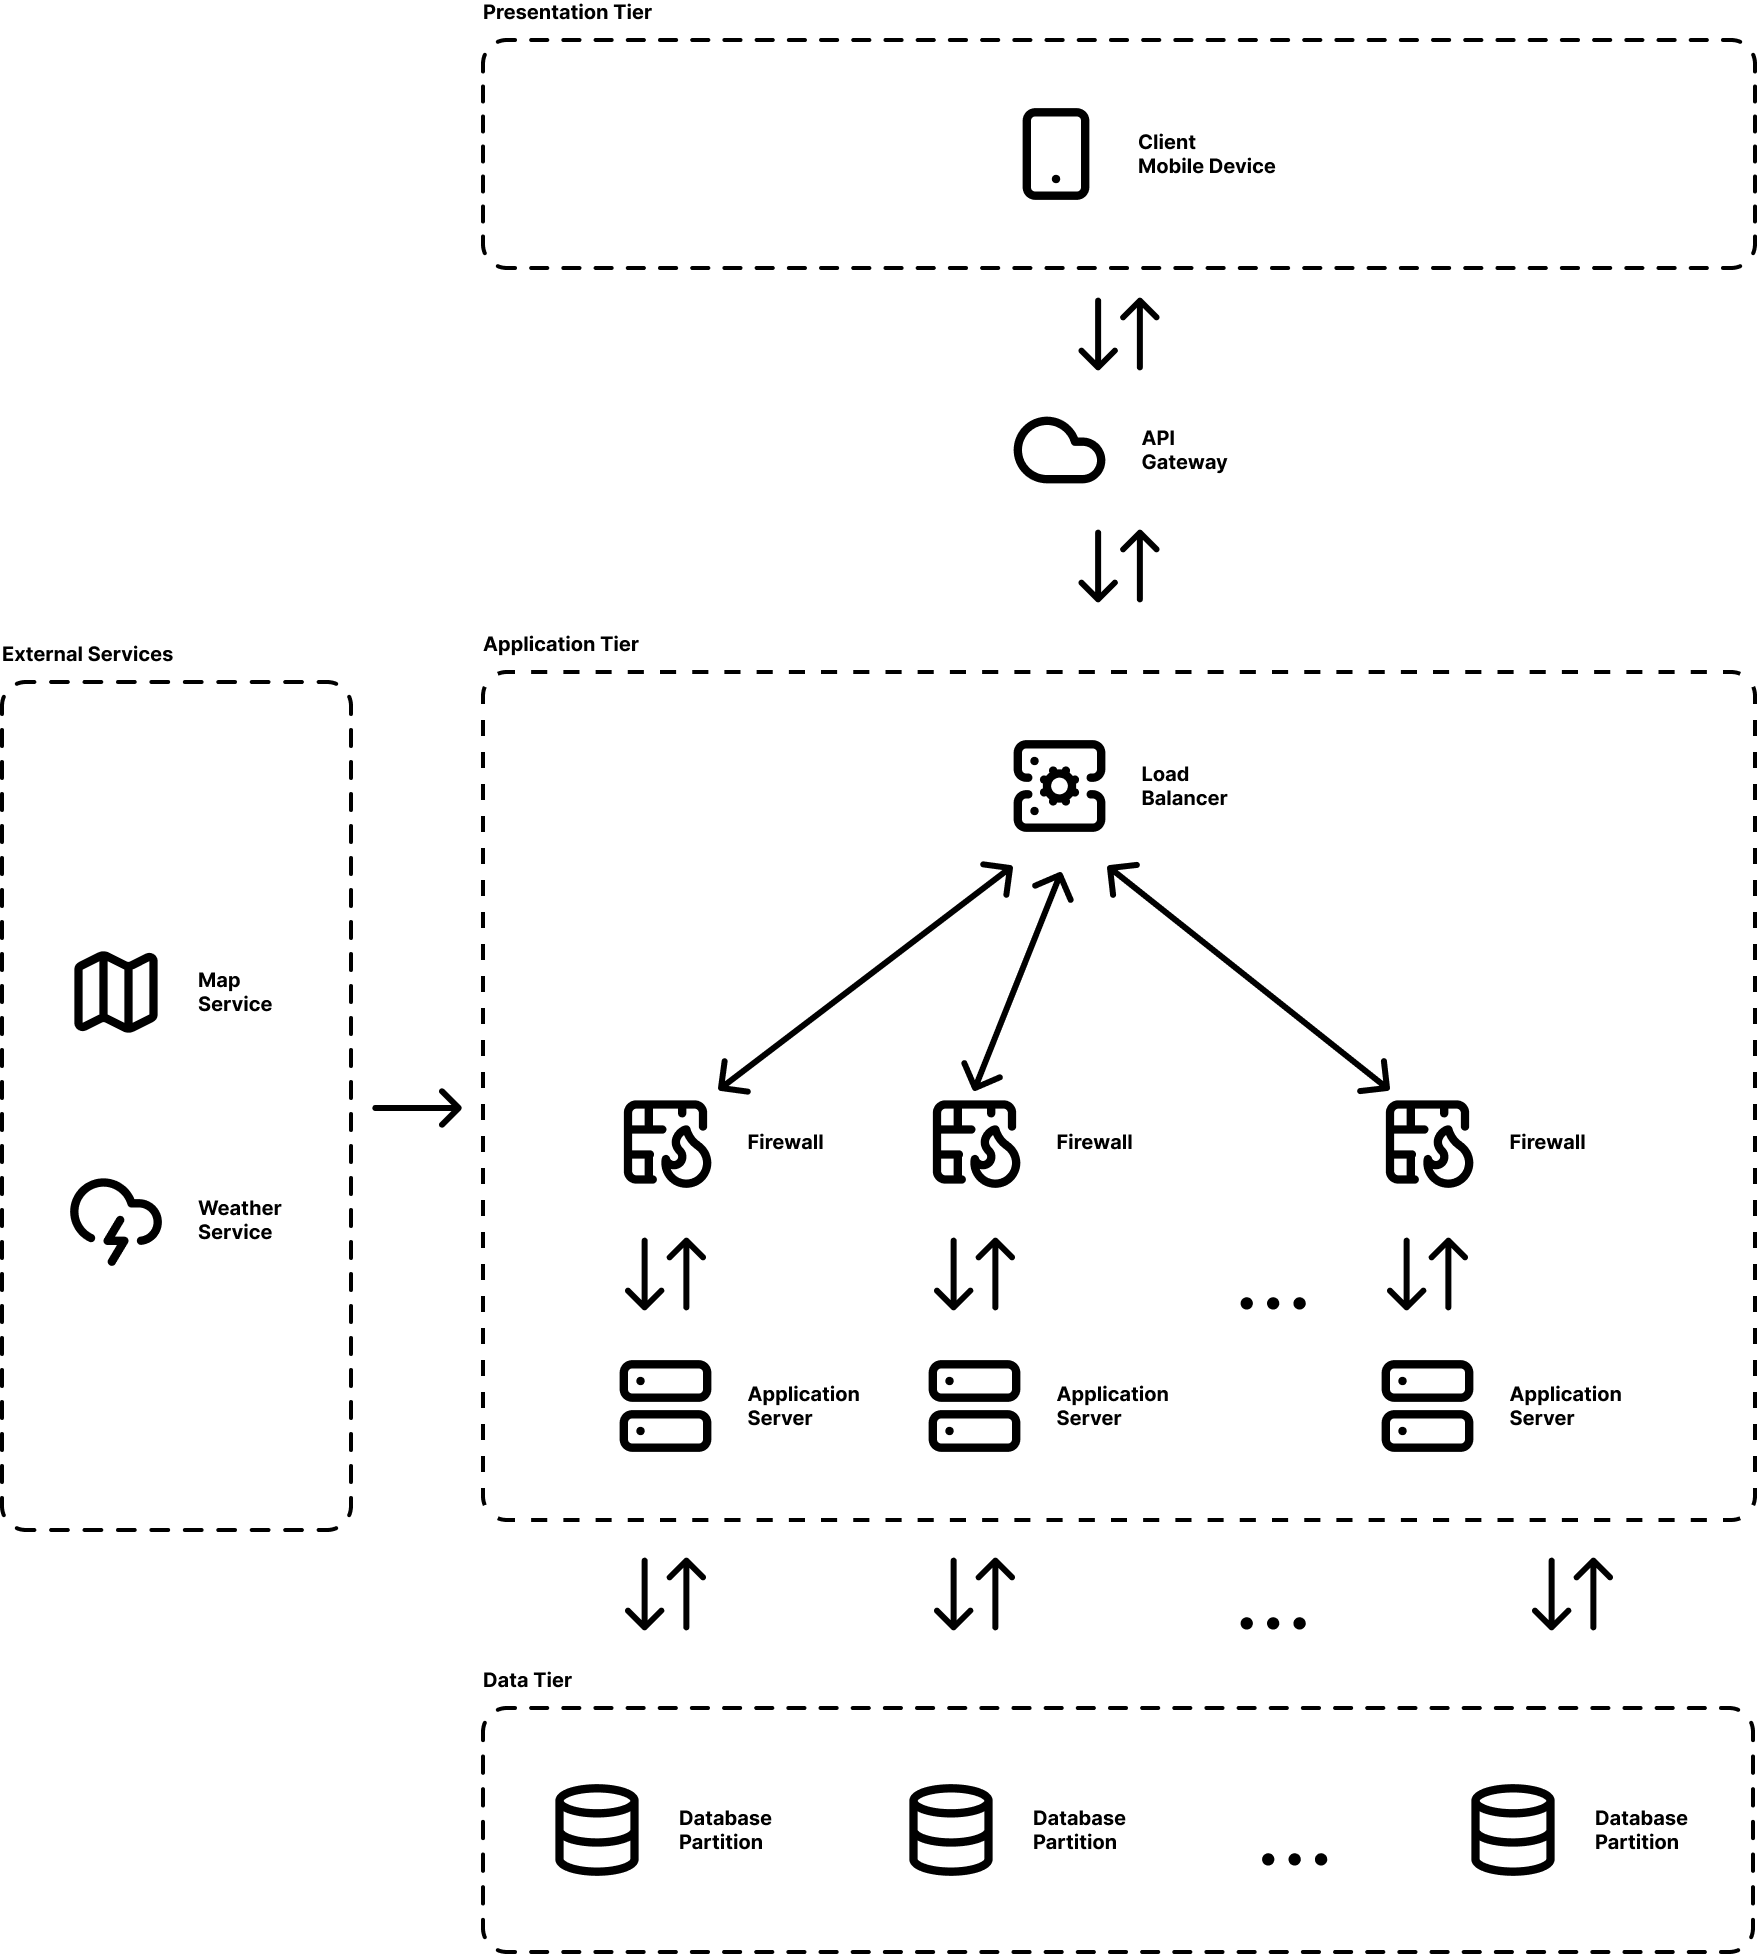
\includegraphics[width=0.7\linewidth]{DD/source/images/diagrams/Detailed System View.png}
    \caption{A more detailed view of the BBP system architecture.}
    \label{fig:detailed_system_view}
\end{figure}

\subsection{Component View}
As already mentioned in the previous section, the BBP system adopts a 3-tier architecture, where the application layer is composed of micro-service components interacting with each other and with external services. 

\subsubsection{Front-end Components}
\paragraph{Mobile Application}
This component acts as the primary user interface, facilitating all user interactions with the platform via HTTPS requests through the API Gateway. It is responsible for the acquisition and transmission of raw data from device sensors and GPS to the back-end, where the data is processed. Additionally, the application implements dynamic view rendering based on authentication state, restricting non-registered users to path exploration features, while providing registered users with all the available functionalities of the platform.

\subsubsection{Application Layer Components}
\paragraph{User Management Service} 
This component acts as the centralized authority for identity and access management. It handles the complete lifecycle of the user, such as registration, authentication and credential management, and session control. Also, it allows users to modify their profile information, change their preferences and completely delete their account. All these functionalities are provided to the user while ensuring compliance with the GDPR-related policies and privacy regulations.

\paragraph{Path Exploration Service} 
The Path Exploration Service allows users to browse the inventory of available bike paths, apply filters, search for routes between departure and destination points, and obtain ranked path results based on predefined scores. It returns detailed path information, including status and summaries of reported obstacles.

\paragraph{Trip Management Service}
This component is responsible for managing the lifecycle of trip data for both planned and completed ones. It implements soft deletion mechanisms to ensure data integrity and view consistency without permanent data loss. Additionally, this service computes performance statistics, such as distance, duration, average speed and other metrics. Crucially, the service enforces strict data isolation, ensuring that trip details and statistics are accessible exclusively to the user who created them.

\paragraph{Report Management Service}
The Reporting component manages both manual and automatic reports as domain entities. In particular it allows publication of reports and validation of automatic report drafts and updates public path information based on the newly published reports, these updates are used to enrich path exploration results and to trigger alert evaluations. Upon publication, the service triggers an update to synchronize and expose the public information of the associated path.

\paragraph{Map \& Weather Adapters}
This component serves as the designated gateway for interactions with external mapping and weather providers. It implements resilience patterns, including timeout handling, fallback strategies, and caching, to ensure system stability. Its primary function is to retrieve weather data to enrich trip information and provides necessary data for map rendering.

\paragraph{Event Bus}
This component is the asynchronous communication backbone, using a publish subscribe model to dispatch domain events. It decouples event ingestion from downstream processing, ensuring high availability and scalability. This component includes buffering capabilities to absorb load spikes and implements reliability patterns such as automatic retries and back-pressure management.

\paragraph{Tracking Ingestion Endpoint}
The Tracking Ingestion Endpoint acts as the entry point for tracking data generated by the user’s device. It receives GPS points or tracking chunks and immediately publishes corresponding tracking events to the event bus, without performing any processing or persistence, ensuring fast acknowledgements and non-blocking ingestion. No processing or persistence is performed at this stage, the only thing that this component does is to transform those data received by the device in event published in the bus and generate an event (write event name here, the receiver of the event and the purpose)

\paragraph{Tracking Processing Worker}
The Tracking Processing Worker consumes tracking events from the event bus, produced by the Tracking Ingestion Endpoint, and performs cleaning, normalization, and validation of the collected data. It handles incomplete or inconsistent sensor readings and communicates with the Automatic Report Generator Worker, sharing data for report generation.

\paragraph{Automatic Report Generator Worker}
The Auto Report Generator Worker reacts to trip completion events. It aggregates processed tracking information and generates automatic report drafts in background, which are later reviewed, validated, and published through the Reporting component.

\paragraph{Alert Service Worker}
The Alert Service Worker listens for contextual updates such as weather changes and newly published obstacle reports. It evaluates these events against predefined severity thresholds and determines their impact on users’ planned trips. When critical conditions are detected, it directly triggers alert notifications for affected users who have requested updates.

For weather-related alerts, the component periodically executes a low-frequency polling mechanism to retrieve meteorological data from external sources through the Map and Weather Integration component. This design choice is motivated by the need to reduce coupling between the alert logic and the weather adapter. Without polling, the weather adapter would be responsible for continuously monitoring weather conditions and actively notifying the Alert Service Worker in case of adverse forecasts, thereby assuming part of the alert evaluation responsibility. By adopting controlled polling, the Alert Service Worker remains the sole component responsible for alert detection logic, while the weather adapter is limited to data retrieval and normalization.

For obstacles alerts, the component listens to the Event Bus for \code{ReportPublished} events and computes a severity score for a planned trip if there's an obstacle inside the report that interests that same trip. 
Whenever the computed severity score for a planned trip exceeds a predefined threshold, the Alert Service Worker sends a notification to the corresponding user, ensuring timely and reactive alert delivery without introducing unnecessary coupling or continuous monitoring overhead in other components.
 

\subsubsection{Data Layer}
\paragraph{Database Management System}
This component acts as a mediator between the components of the application layer and the databases. It is responsible for managing all domain data, including user profile data and preferences, path information, planned and completed trips, tracking data, reports and any other aggregated data required for proper functioning of the system.

\subsubsection{External Services}
\paragraph{Map Service}
This component is a third-party geographical data provider used by the platform. It supplies the assets for map visualization (vector or raster tiles) and other geographical features.

\paragraph{Weather Service}
This component is a third-party meteorological data provider used by the platform. It supplies access to the current atmospheric conditions, and severe weather warnings for specific geospatial coordinates. This data is consumed via API to enrich trip details and trigger safety alerts for users.

\paragraph{User Device}
This component is the physical hardware interface and operating system services of the user's mobile device. It serves as the primary source of telemetry, continuously generating geolocation coordinates (via GPS) and motion sensor data. Crucially, it enforces operating system-level security, ensuring that the application can only access this sensitive hardware if the user has explicitly granted the necessary runtime permissions.

\begin{figure}[H]
    \centering
    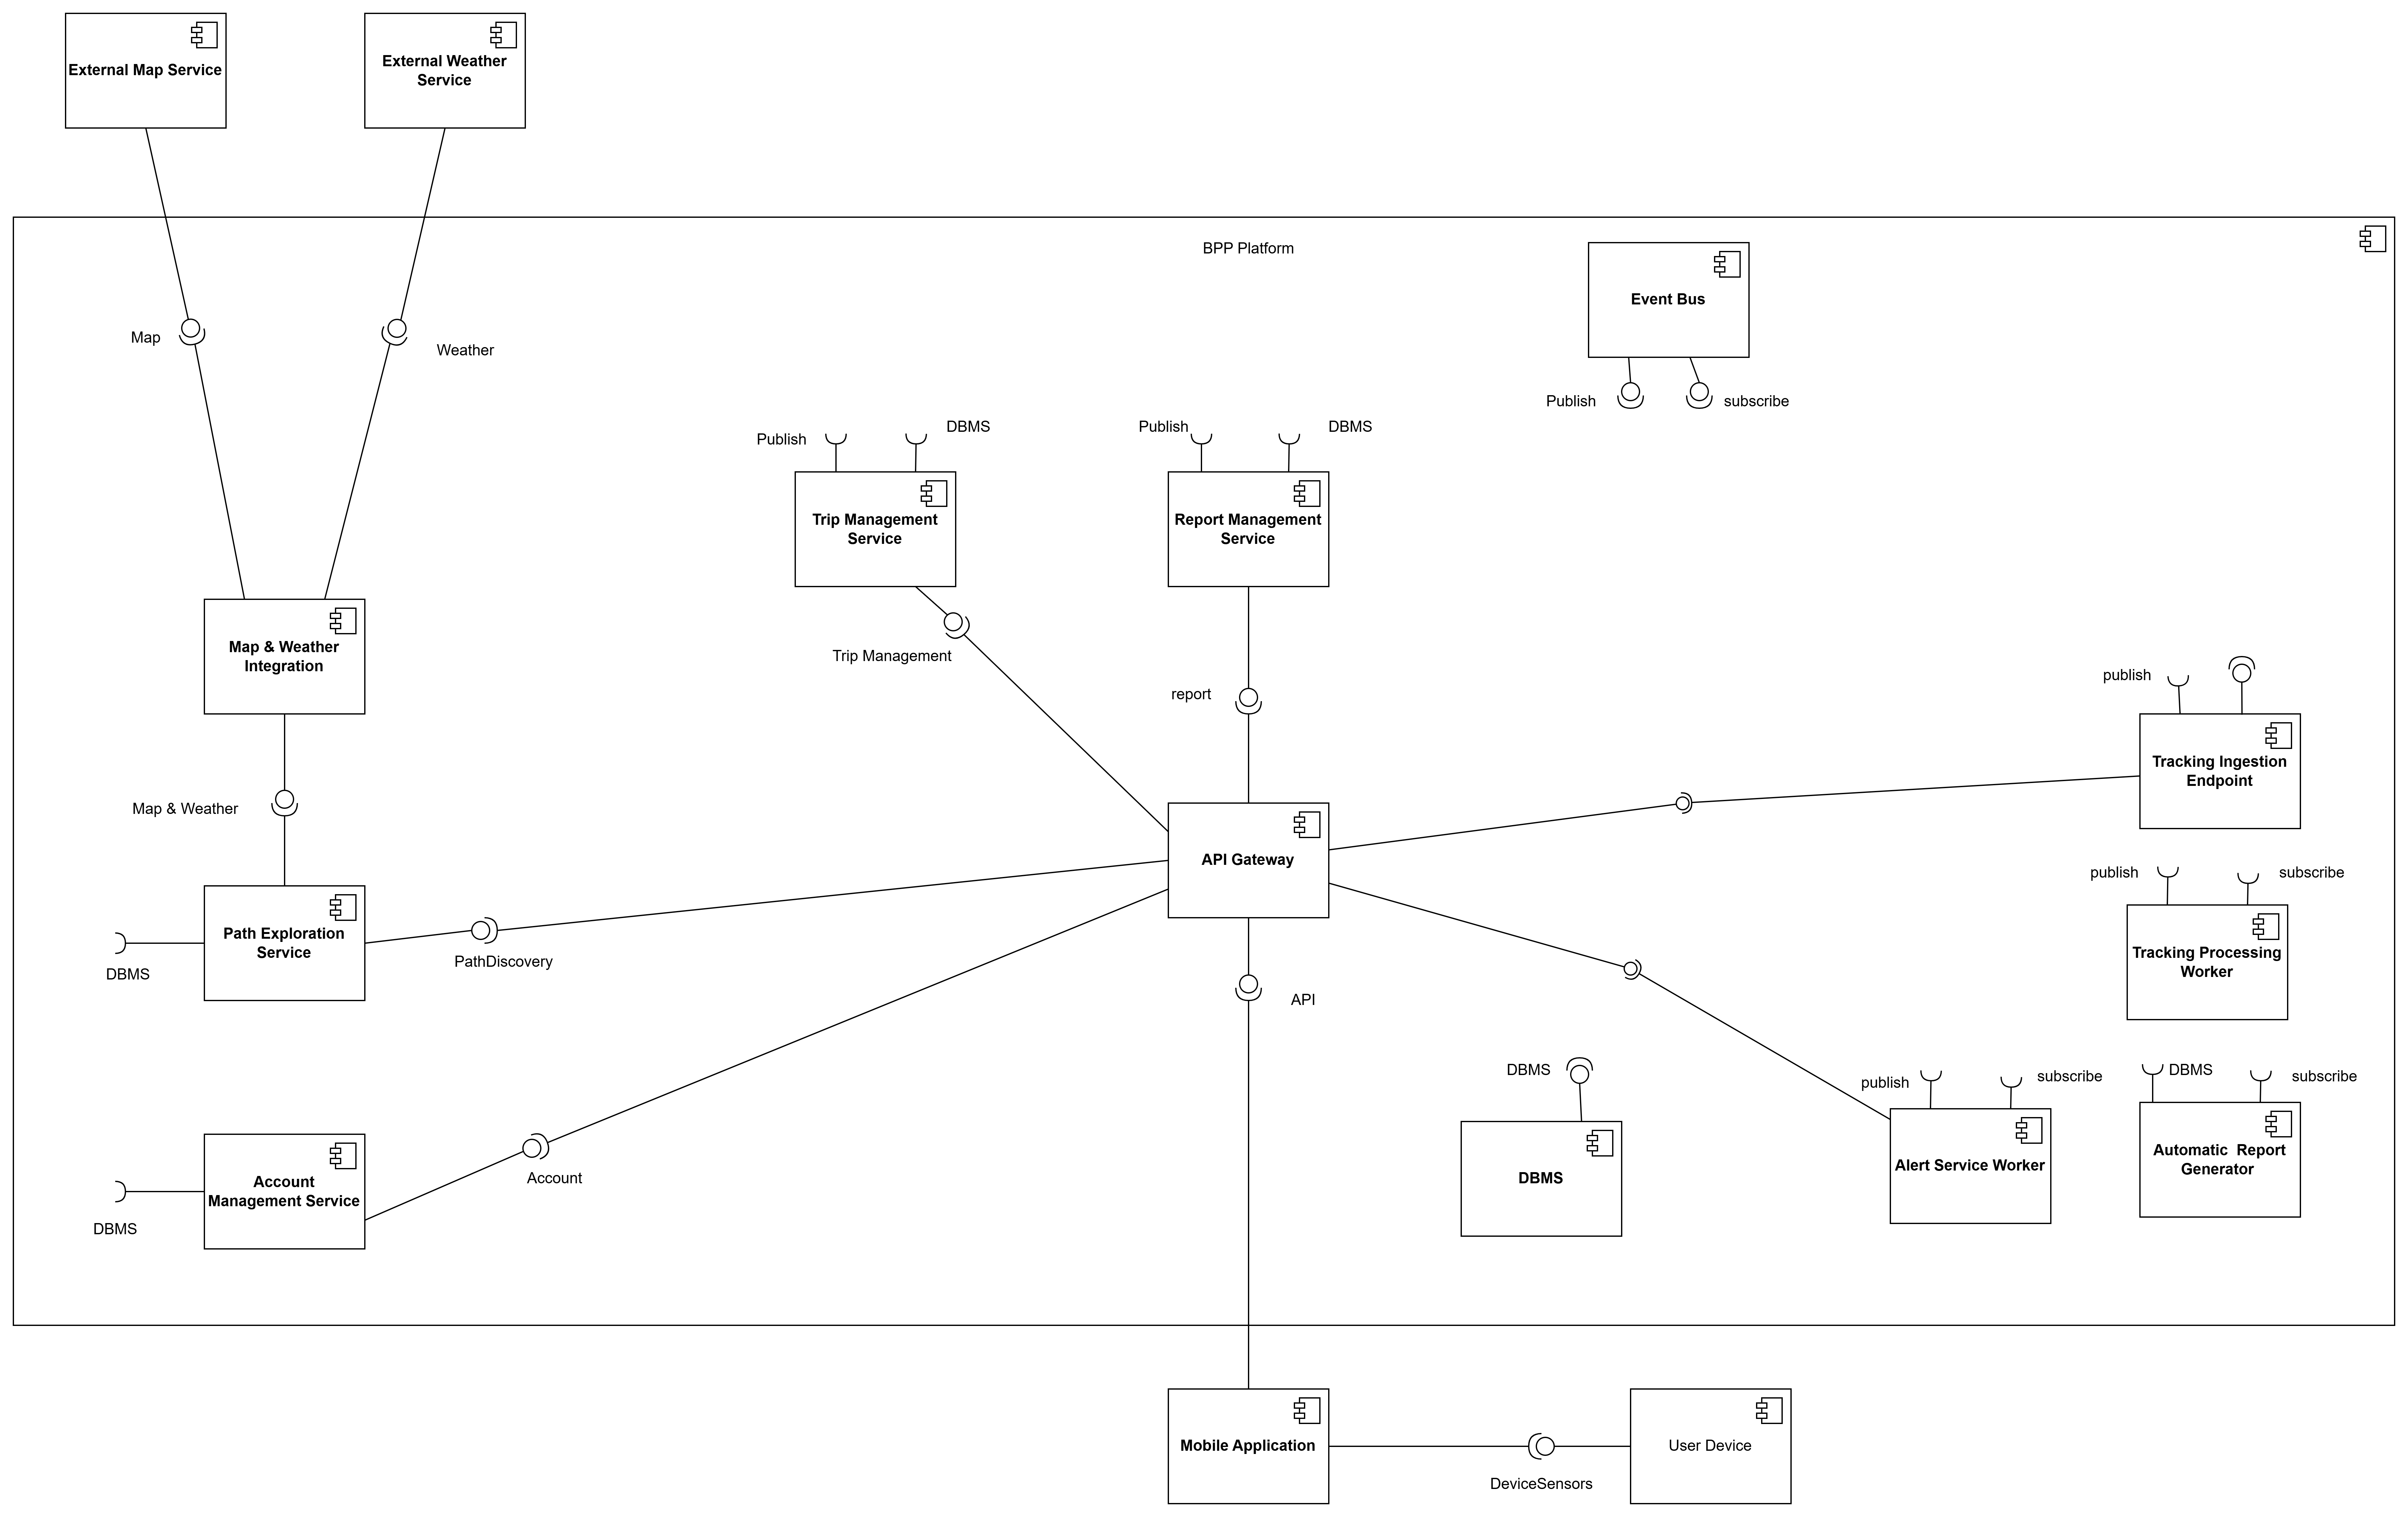
\includegraphics[width=0.9\linewidth]{DD//source//images//diagrams/component_diagram.png}
    \caption{Component Diagram.}
    \label{fig:component_diagram}
\end{figure}

\subsection{Deployment View}
\begin{figure}[H]
    \centering
    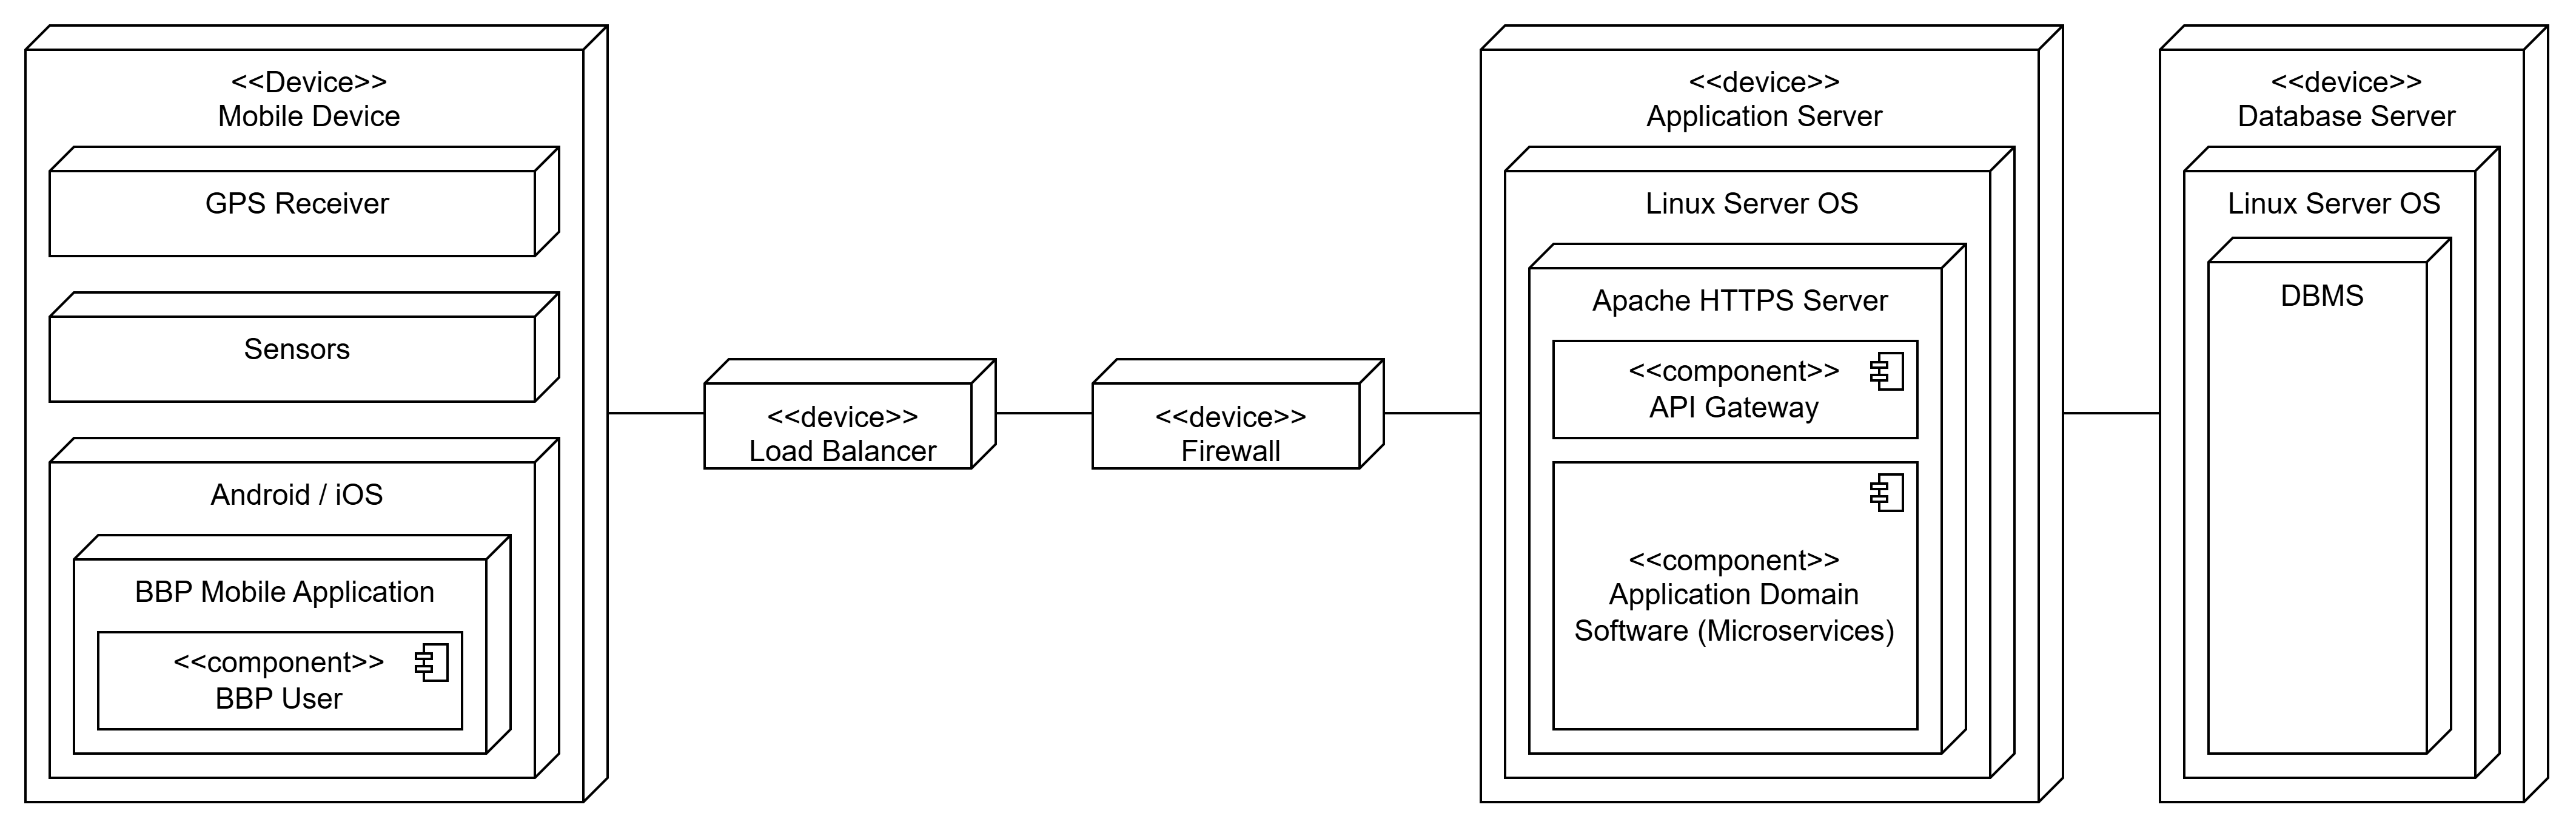
\includegraphics[width=0.9\linewidth]{DD//source//images//diagrams/System Deployment View.png}
    \caption{System Deployment View.}
    \label{fig:system_deployment_view}
\end{figure}

\paragraph{Mobile Device}
The device is used by the BBP users to access the platform, via the mobile application. The user is required to download the application from centralized distribution channels like Google Play Store (for Android) or App Store (for iOS), in order to interact with the system. Also, the device is responsible for gathering all the GPS and sensor data, required for the correct functioning of specific features of the application. 

All data exchange between the mobile client and the server infrastructure is encapsulated over HTTPS, passing through a load balancer, for high availability, and firewalls, for robust security. Requests are finalized at the API Gateway, which acts as the single entry point for the back-end, handling request routing, rate limiting, and authentication before passing data to the internal application servers.

\paragraph{Load Balancer}
The load balancer acts as a reverse proxy, distributing incoming network traffic across the servers that constitute the application layer. Its primary purpose is to ensure high availability and reliability by preventing that a single server may become a point of failure or a performance bottleneck, slowing down the entire system.

\paragraph{Firewall}
The firewall is a network security system that acts as a protective barrier between the trusted internal network (BBP platform back-end) and the untrusted external network. Its primary purpose is to monitor and control incoming and outgoing traffic based on predetermined security rules to prevent unauthorized access and block malicious data. Notoriously, the deep packet inspection required by the firewall represents a potential performance bottleneck. Therefore, the firewall is strategically positioned after the load balancer to reduce the volume of packets it has to inspect.

\paragraph{Application Server}
The application server handles all the incoming requests from users interacting with the platform via the mobile application. It is responsible for processing data sent by the client and ensures data persistence by interacting with the DBMS via TCP/IP. It also integrates information coming from external services with which it communicates via HTTPS.

\paragraph{Database Management System Server}
The database runs on a clustered architecture to ensure high availability and data consistency. This configuration guarantees that all nodes maintain identical dataset and that the application server is updated with the latest information, preventing errors caused by data mismatches between nodes.

\subsection{Runtime View}
The following diagrams show the interaction between the various component that make up the BBP system. Note that the message flow modelled by these sequence diagrams do not include all the possible exceptions the system can run into for a matter of simplicity. Furthermore, as already mentioned before, every interaction between the client and the server is mediated by the API Gateway component, which also has caching mechanisms and acts as a session handler for registered users. These functionalities are not shown in the diagrams to make them more readable.

\vspace{0.5cm}\noindent
\textbf{UC1: User Registration}
\begin{figure}[H]
    \centering
    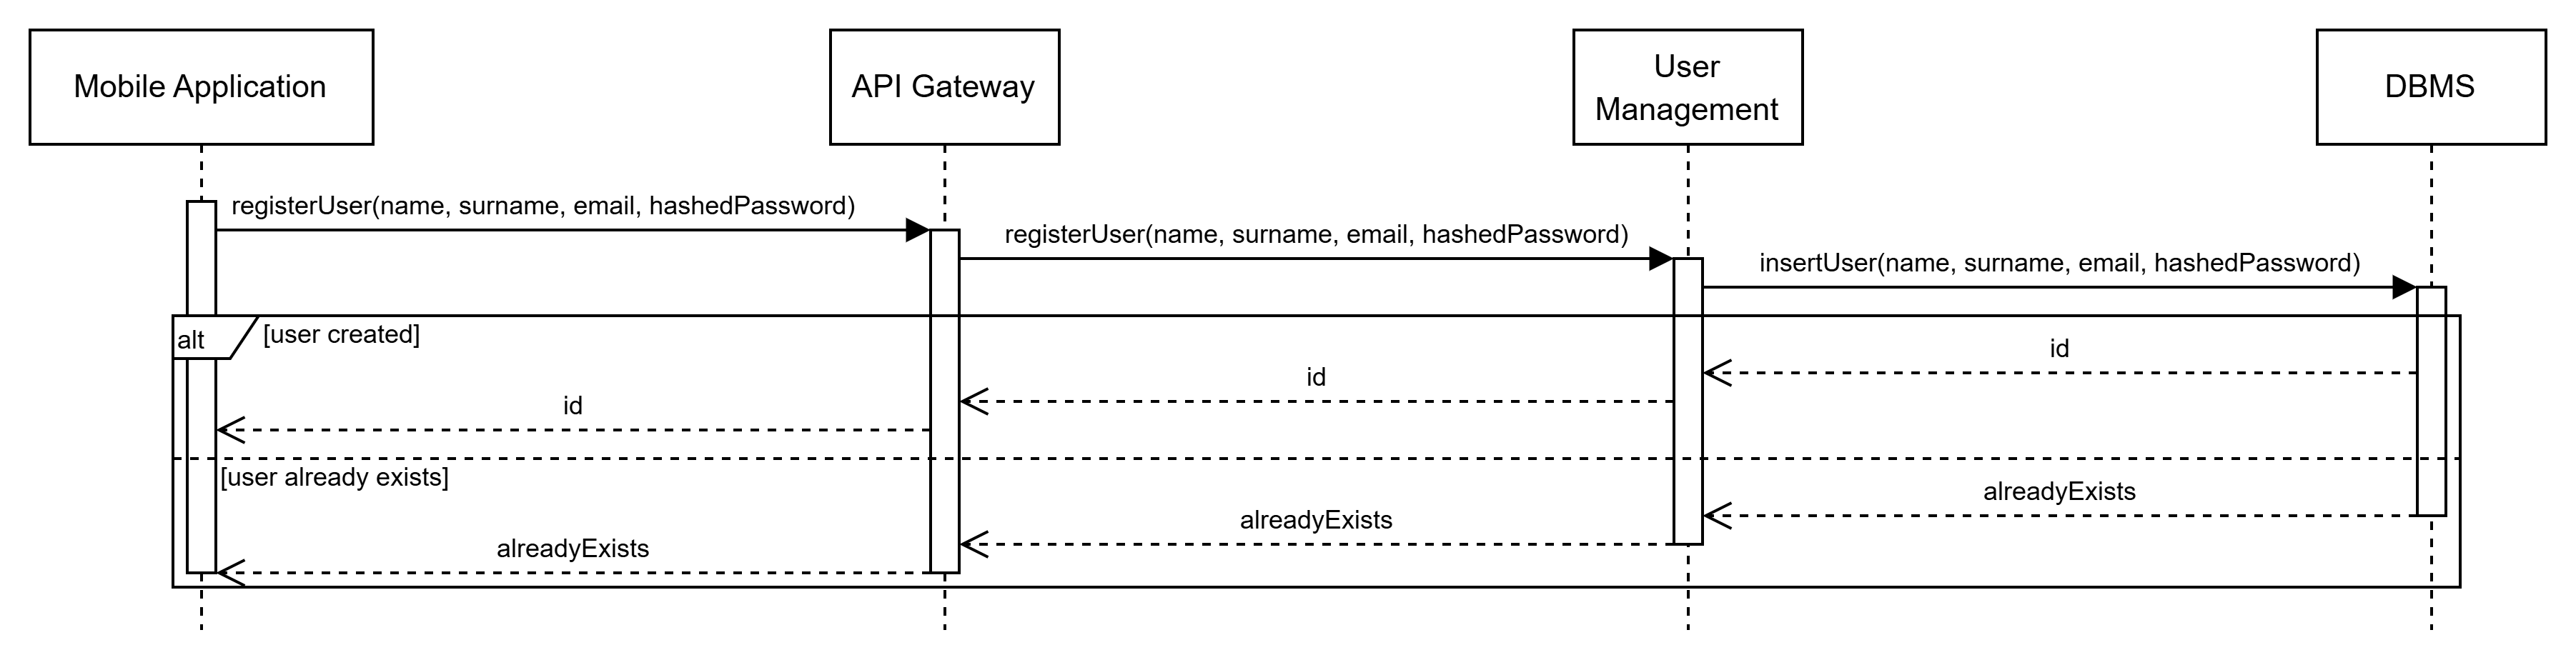
\includegraphics[width=\linewidth]{DD//source//images//diagrams//sd_registration.png}
    \caption{User Registration Sequence Diagram.}
    \label{fig:registration_sd}
\end{figure}

This sequence diagram shows the interactions between system components during user registration. Note that the local email and password validation is only syntactical, checking for errors in the email formatting and for well formed passwords. The password is hashed using salting and peppering, as already mentioned in the RASD, before sending the registration request to the back-end for better security. The \code{id} is generated by the DBMS, cached in the API gateway and returned to the user for session handling: all subsequent client requests also include the id, so the API gateway can authenticate the user.

\vspace{0.5cm}
\noindent
\textbf{UC2: User Login}
\begin{figure}[H]
    \centering
    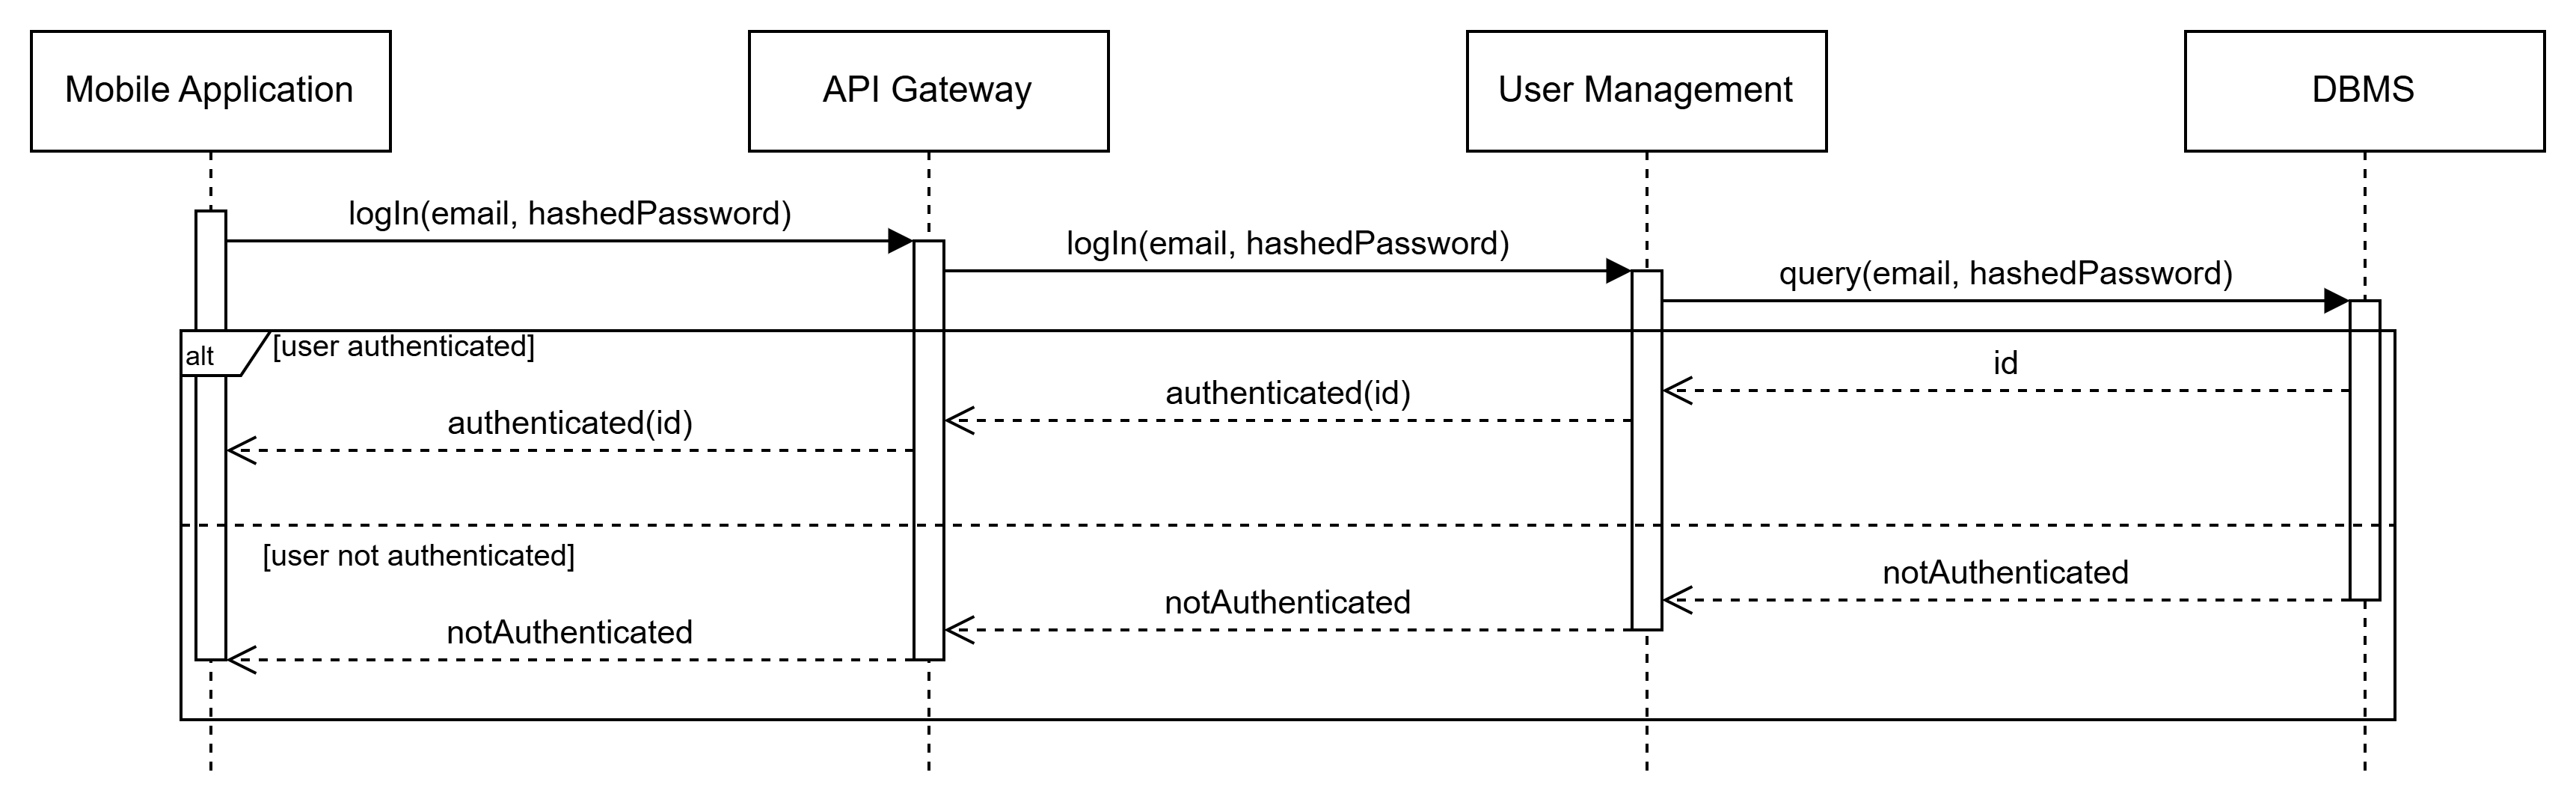
\includegraphics[width=\linewidth]{DD//source//images//diagrams/sd_login.png}
    \caption{User Login Sequence Diagram.}
    \label{fig:sd_login}
\end{figure}

This sequence diagram shows the interactions between system components during user login. If the email and hashed password correspond to an entry of the database, the corresponding id is cached in the API gateway and returned to the client, so all subsequent requests can be authenticated.

\vspace{0.5cm}
\noindent
\textbf{UC3: Update Profile Data}
\begin{figure}[H]
    \centering
    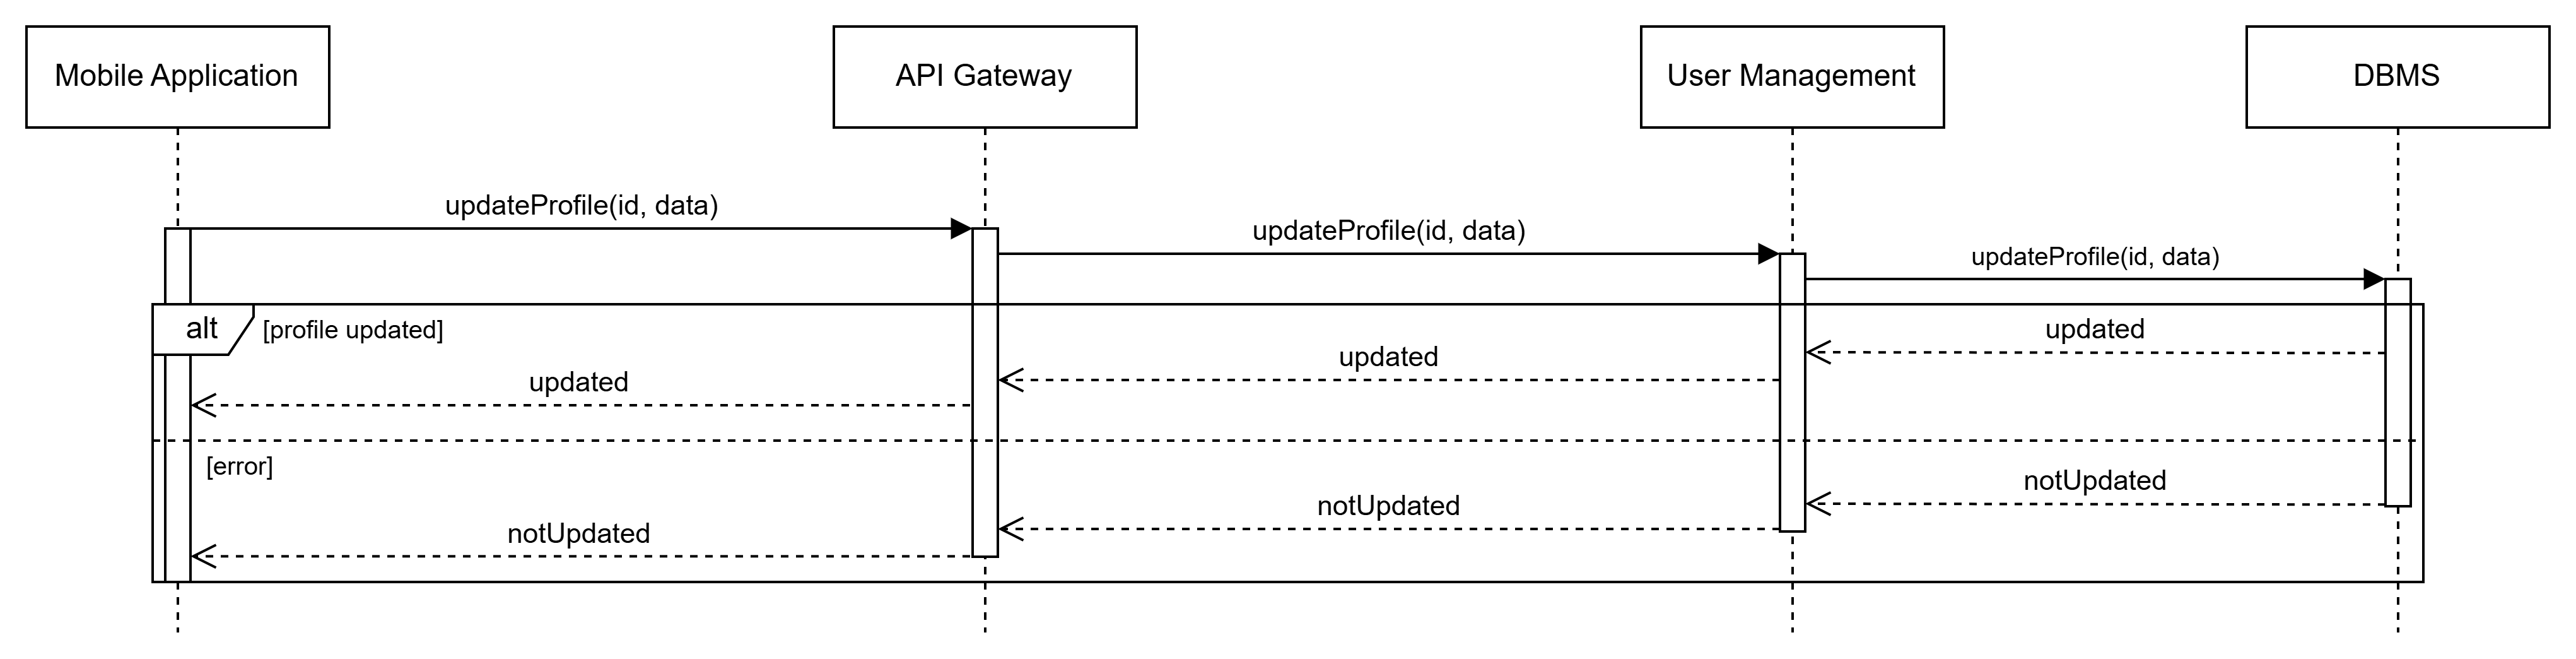
\includegraphics[width=\linewidth]{DD//source//images//diagrams/sd_update_profile.png}
    \caption{Update Profile Data Sequence Diagram.}
    \label{fig:update_sd}
\end{figure}

This sequence diagram shows the interactions between system components during profile data updates. The client sends an update request to the server, which then responds with a success or failure message.

\newpage \noindent
\textbf{UC4: Delete Account}
\begin{figure}[H]
    \centering
    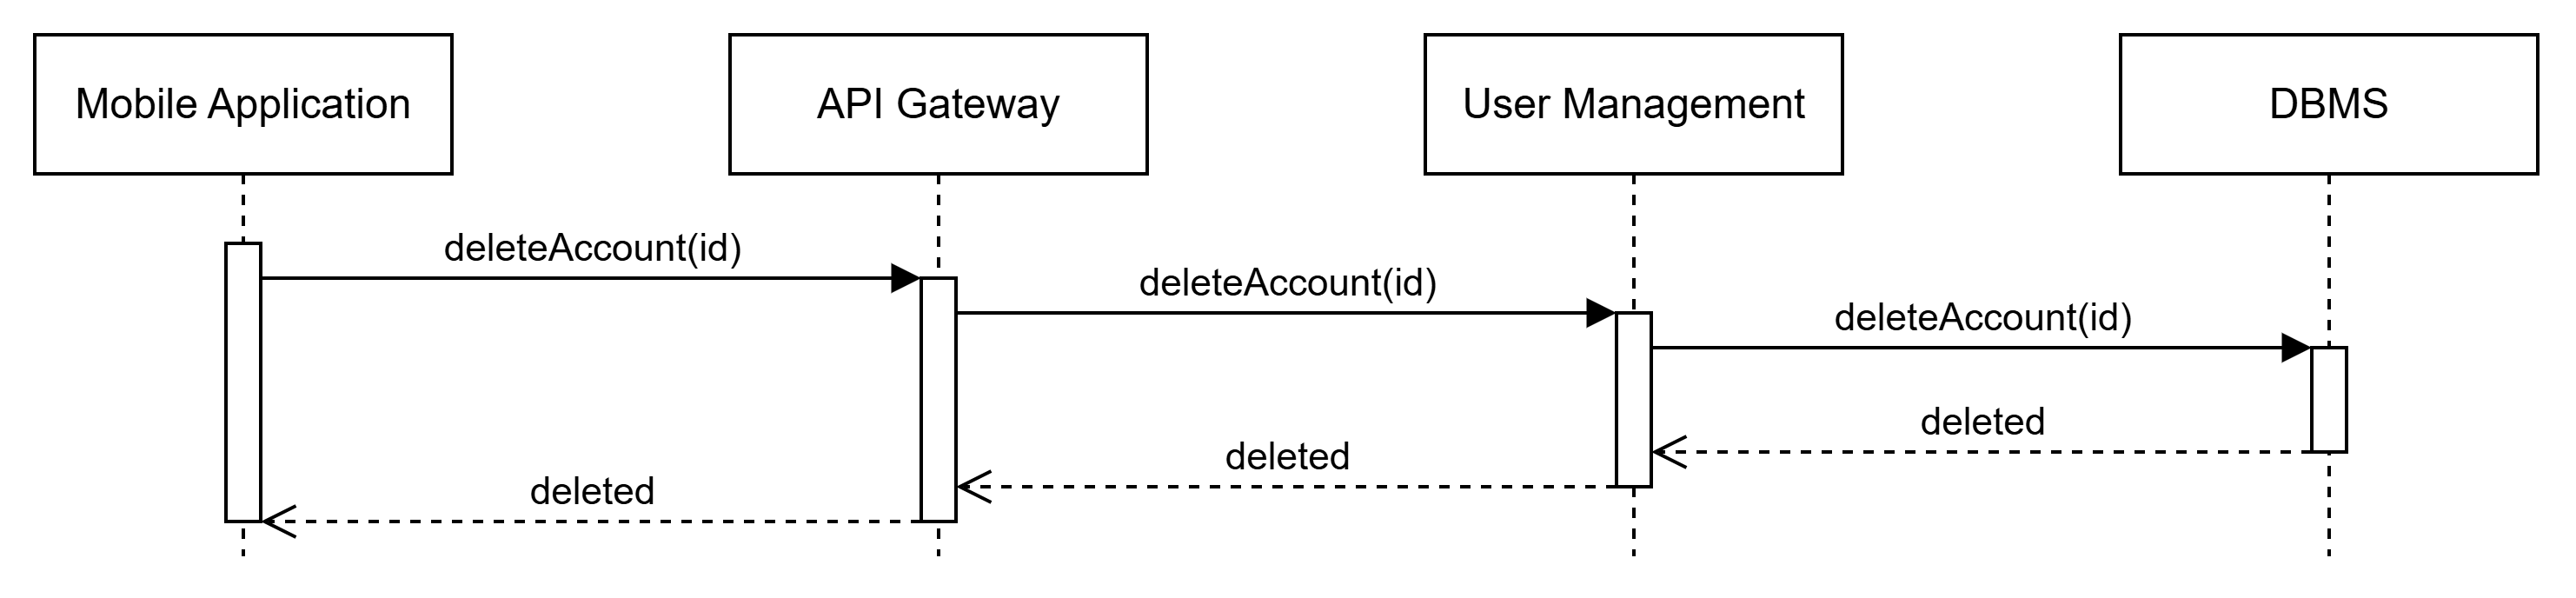
\includegraphics[width=\linewidth]{DD//source//images//diagrams/sd_delete_account.png}
    \caption{Delete Account Sequence Diagram.}
    \label{fig:delete_sd}
\end{figure}

This sequence diagram shows the interactions between system components during account deletion. By GDPR regulations, all sensitive information regarding the user is deleted, while all reports he compiled are persisted in the database.

\newpage
\noindent
\textbf{UC5: Browse Bike Paths}
\begin{figure}[H]
    \centering
    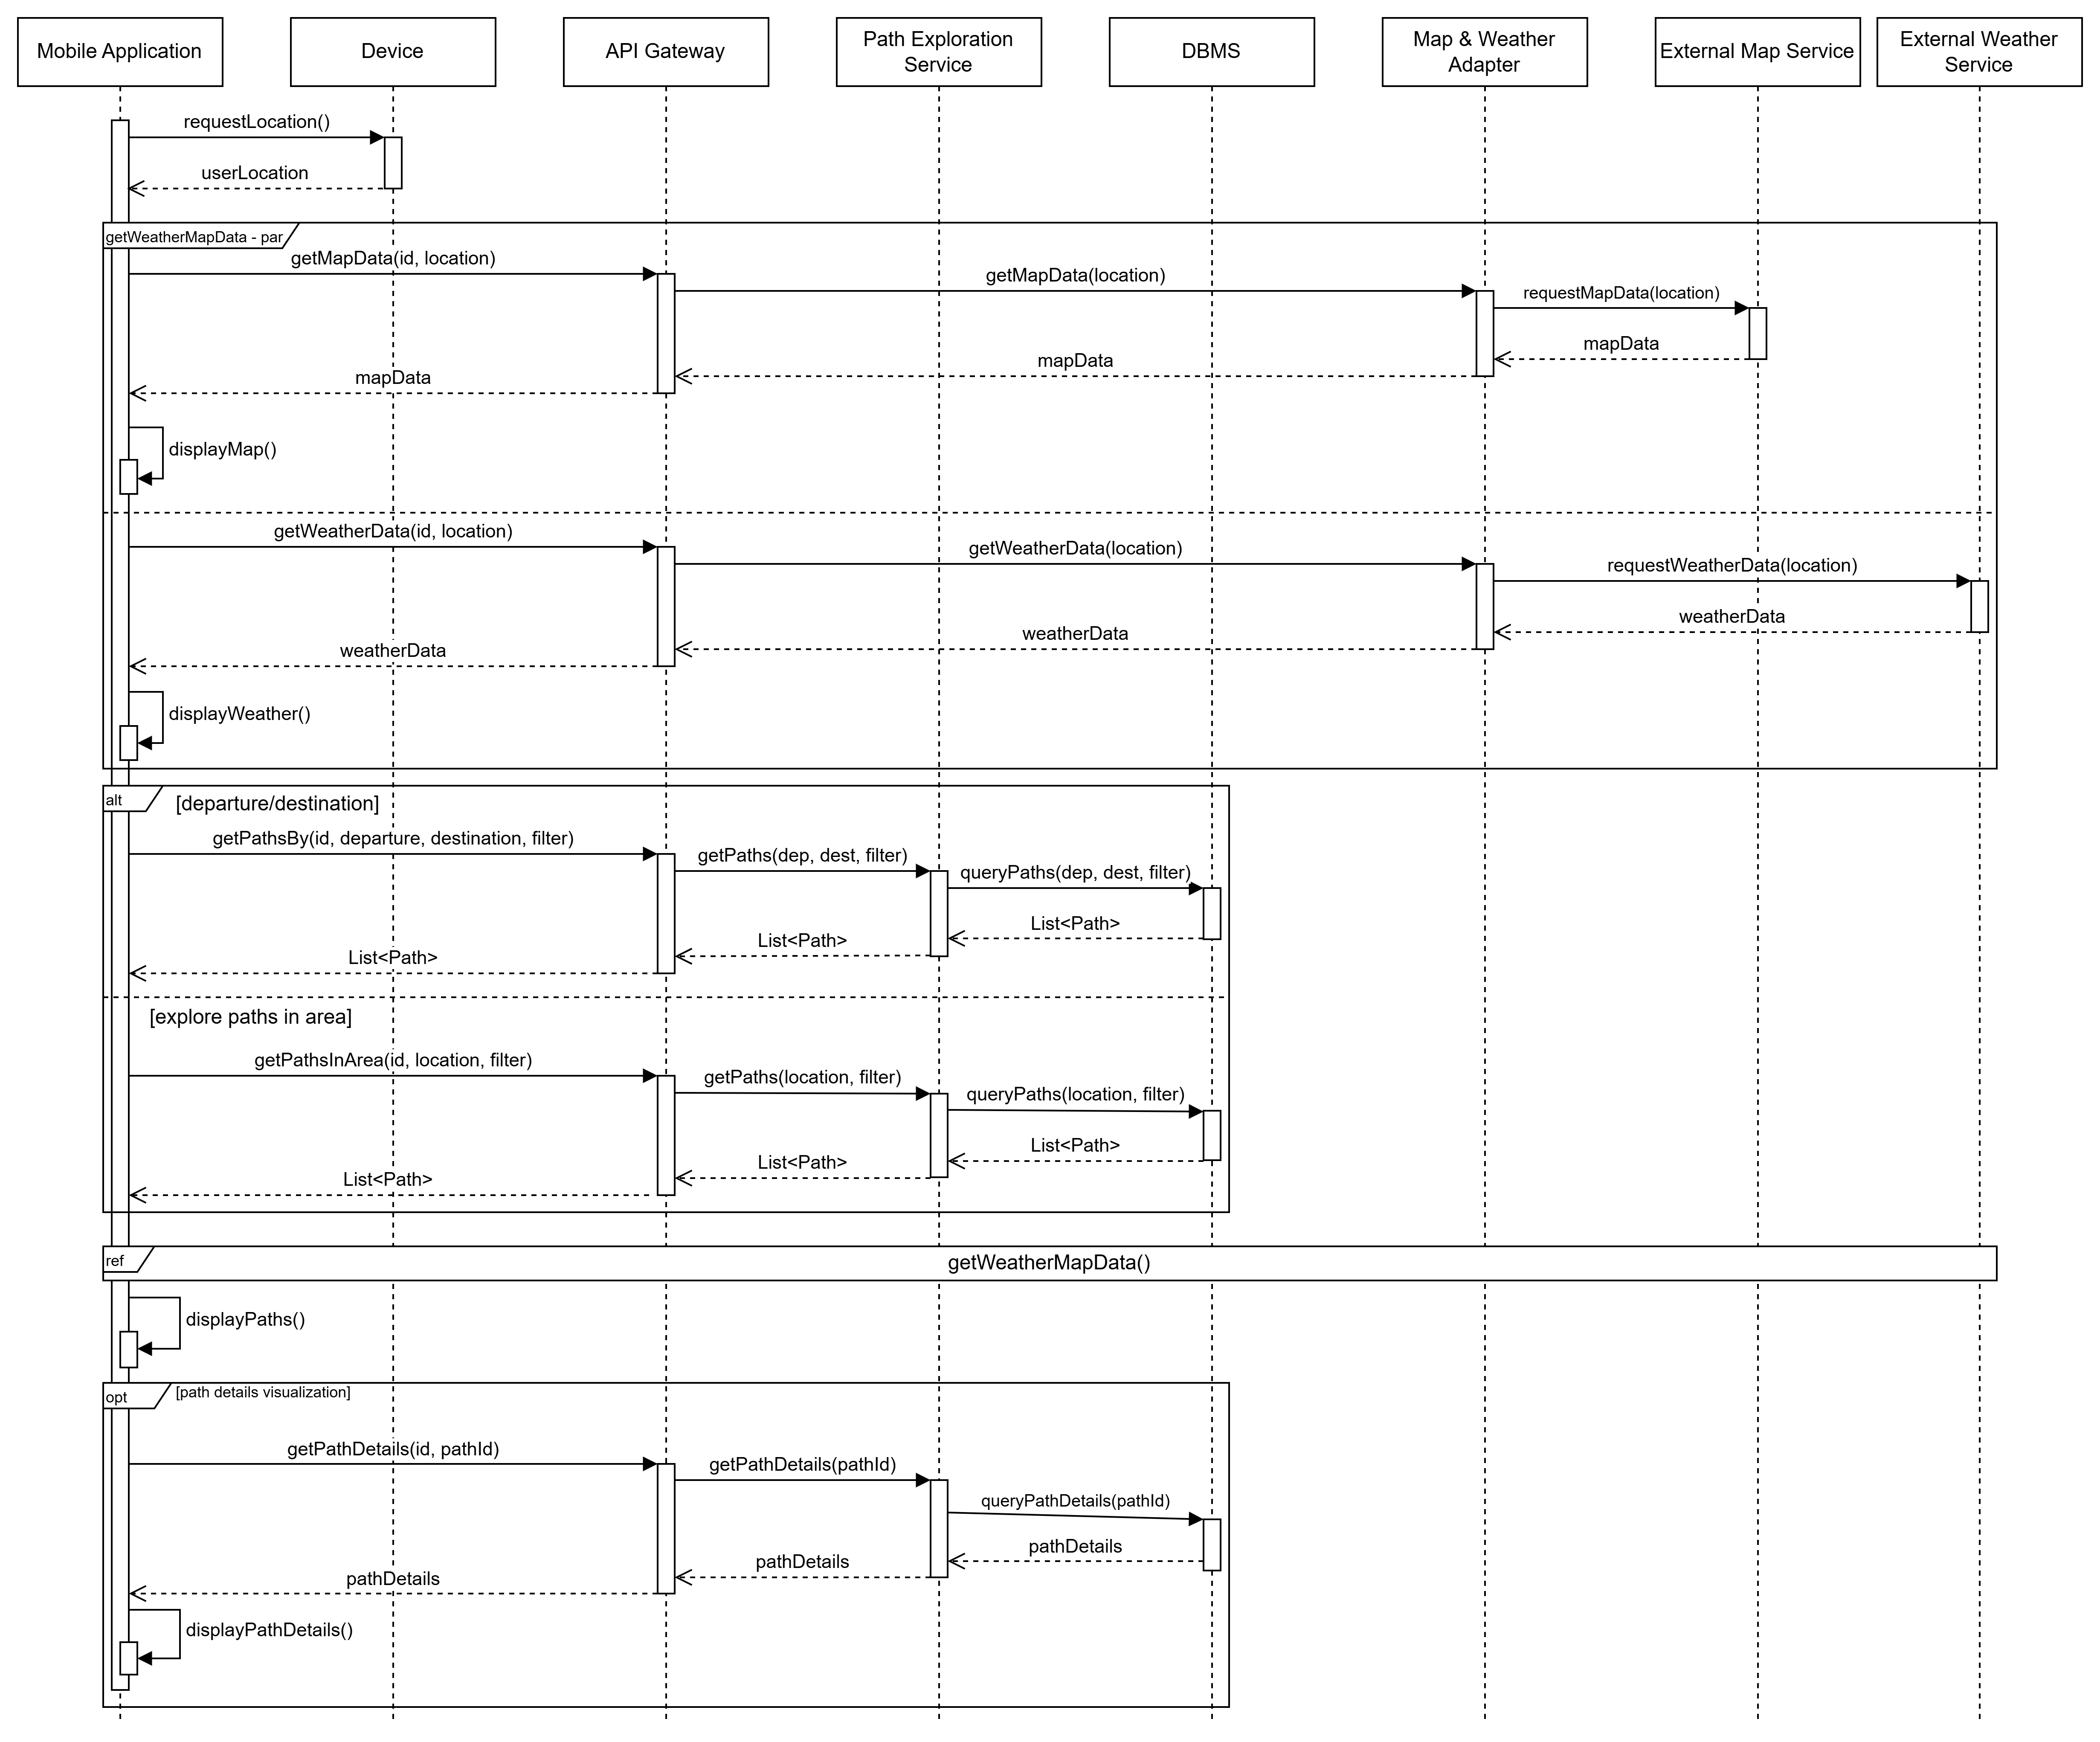
\includegraphics[width=\linewidth]{DD//source//images//diagrams/sd_browse.png}
    \caption{Browse Bike Paths Sequence Diagram.}
    \label{fig:browse_sd}
\end{figure}


This sequence diagram shows the interactions between system components during bike paths browsing. Once the user navigates to the dedicated section in the mobile application, a location request to the device is dispatched. When the user location is returned by the device, the application gets map information from the external service, in order to display the map on the screen. If the user inserts departure and destination points, with attached filters, a request to the server is dispatched, which returns the list of the available bike paths, ranked by score. Otherwise, if the user explores the map, a request by area is sent to the server. In both cases, the map information is updated and the bike paths are displayed.

The user can optionally visualize the details of a given path by clicking on it, which not only retrieves all the path information, but also the weather information on the area regarding the bike path.

\newpage
\noindent
\textbf{UC6: Plan Trips}
\begin{figure}[H]
    \centering
    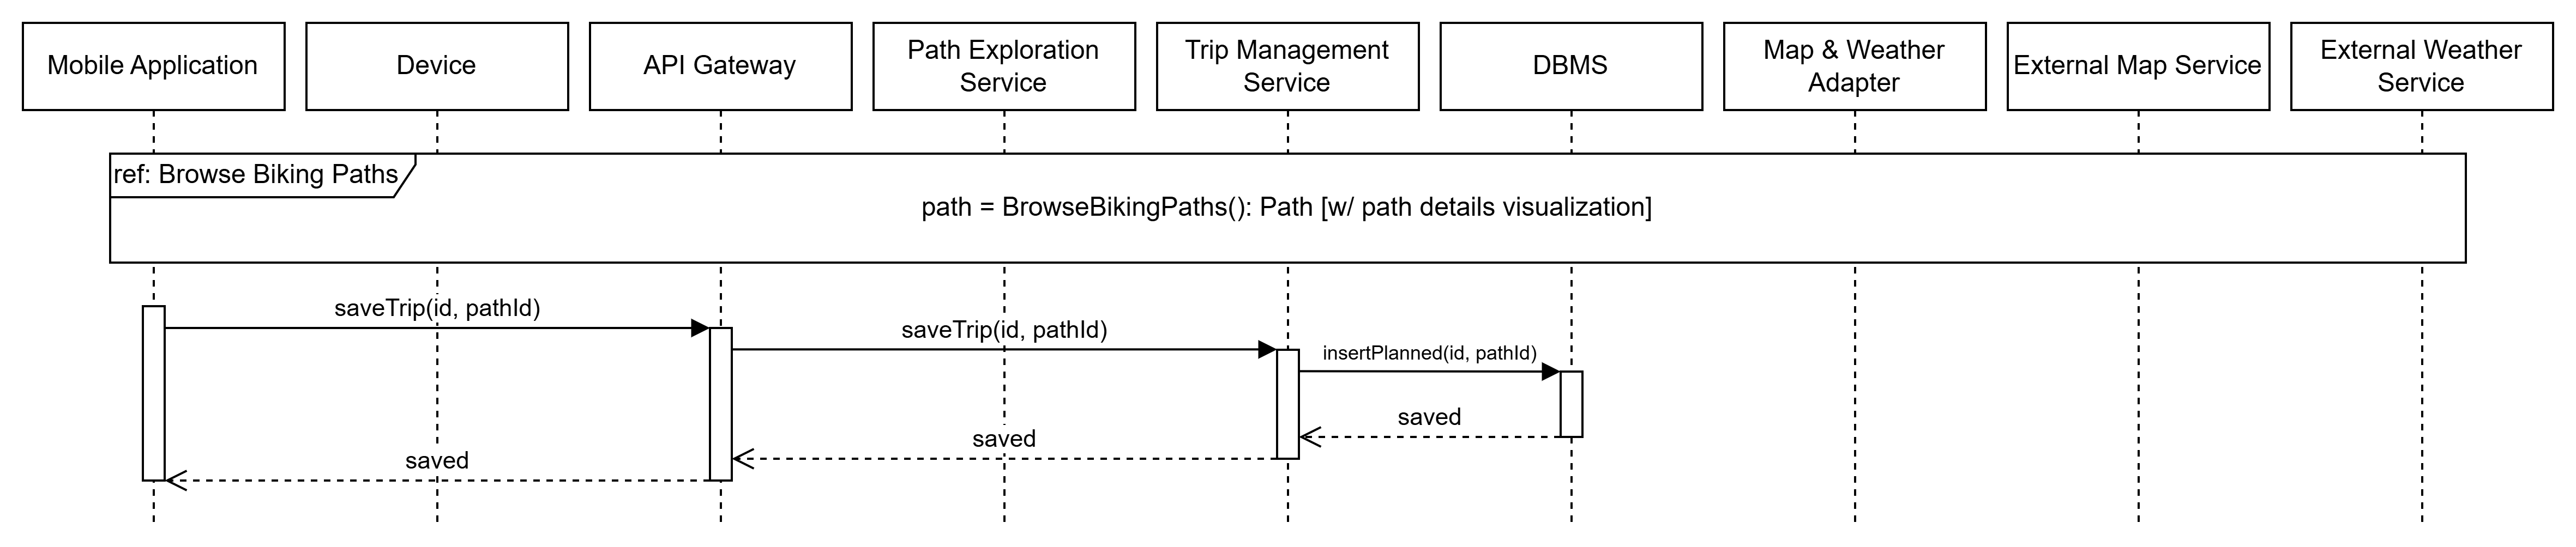
\includegraphics[width=\linewidth]{DD//source//images//diagrams/sd_plan.png}
    \caption{Plan Trips Sequence Diagram.} 
    \label{fig:plan_sd}
\end{figure}
This sequence diagram shows the interactions between system components during trip planning. After browsing and selecting a bike path, the user can decide to save the trip: the client sends a request to the trip management service, which saves the trip in the database via the DBMS. 

\vspace{0.5cm}\noindent
\textbf{UC7: Change Automatic Tracking Settings}
\begin{figure}[H]
    \centering
    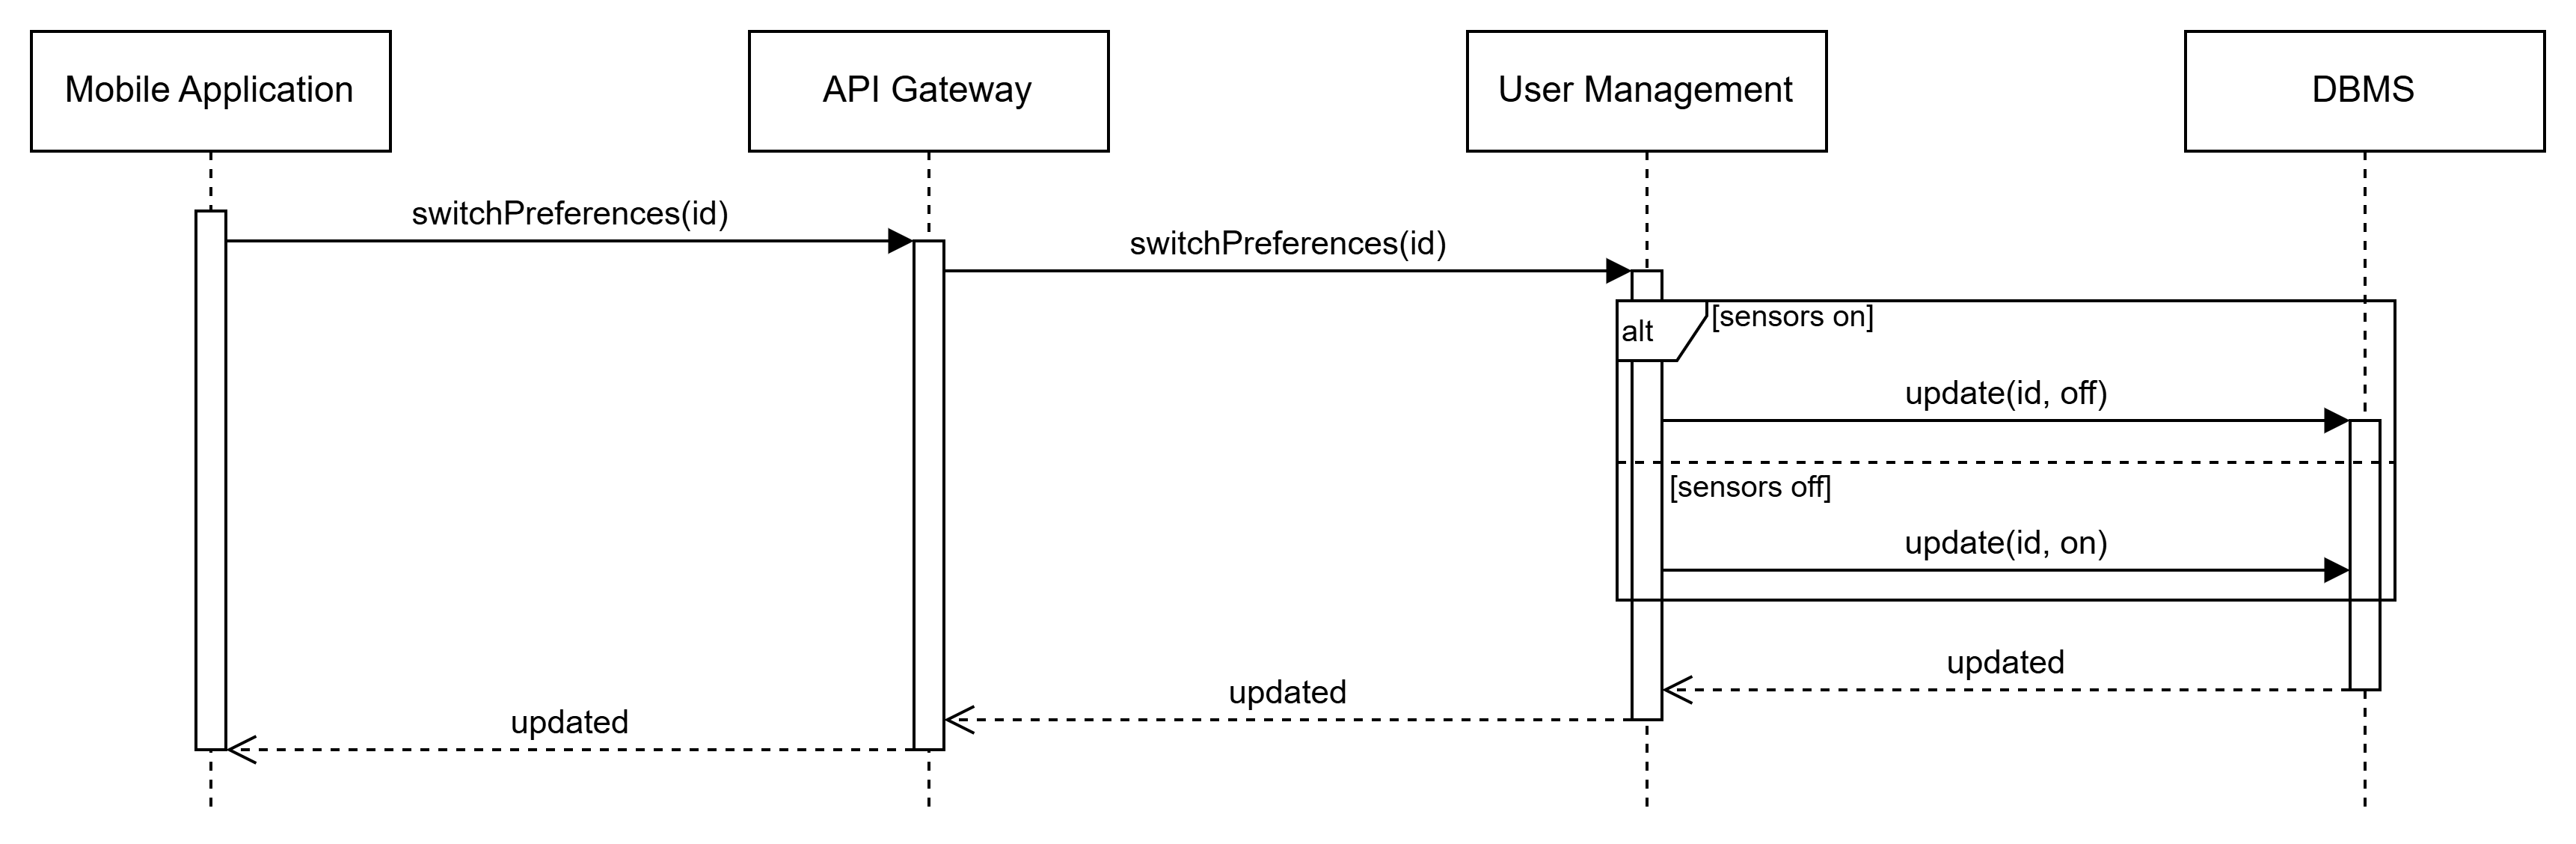
\includegraphics[width=\linewidth]{DD//source//images//diagrams/sd_change_pref.png}
    \caption{Change Automatic Tracking Settings Sequence Diagram.}
    \label{fig:change_prefs_sd}
\end{figure}

This sequence diagram shows the interactions between system components during preferences changes. The client simply dispatches a request to switch preferences to the user management component, which saves the preferences to the database, via the DBMS.

\newpage
\noindent
\textbf{UC8: View History and Statistics of Completed Trips}
\begin{figure}[H]
    \centering
    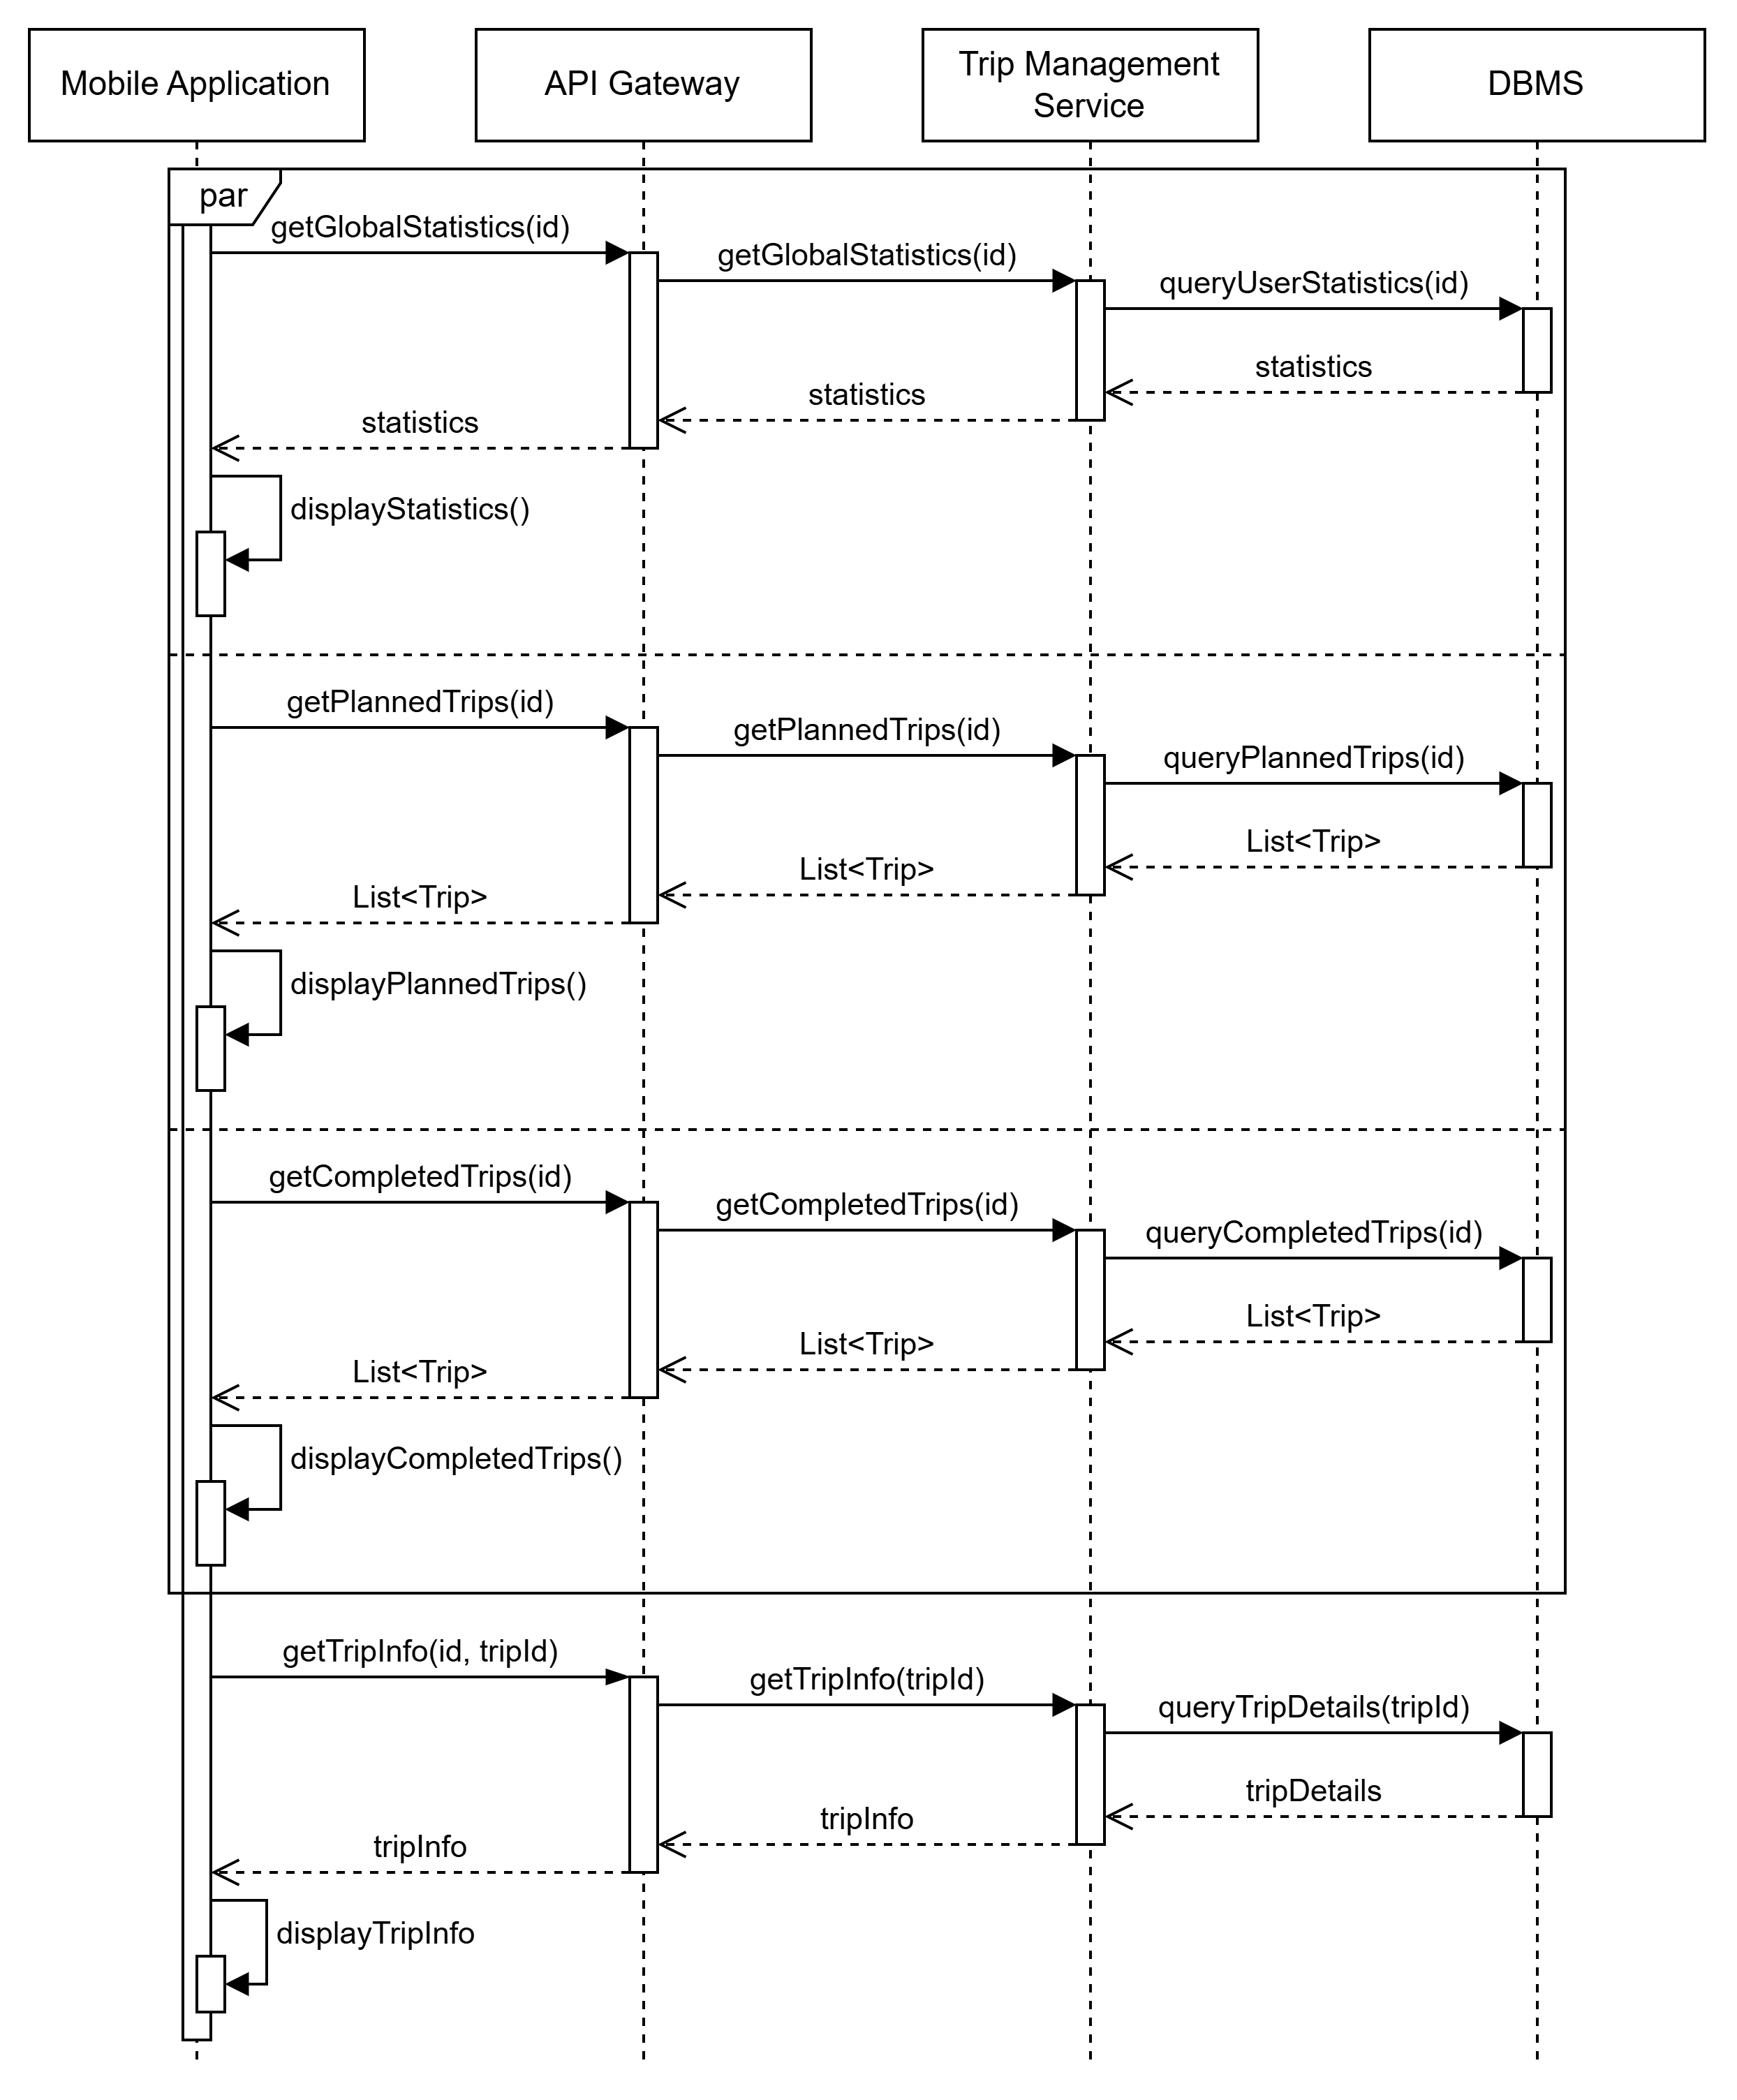
\includegraphics[width=0.9\linewidth]{DD//source//images//diagrams/sd_details.png}
    \caption{View History and Statistics of Completed Trips Sequence Diagram.}
    \label{fig:details_sd}
\end{figure}

This sequence diagram shows the interactions between system components when the user views the history and statistics of completed trips. The client gets from the server the global user statistics, all planned and completed trips in parallel, showing them to the user. Once the user clicks on a completed trip, all information regarding the trip is fetched and displayed.

\newpage
\noindent
\textbf{UC9: Delete Trips from History}
\begin{figure}[H]
    \centering
    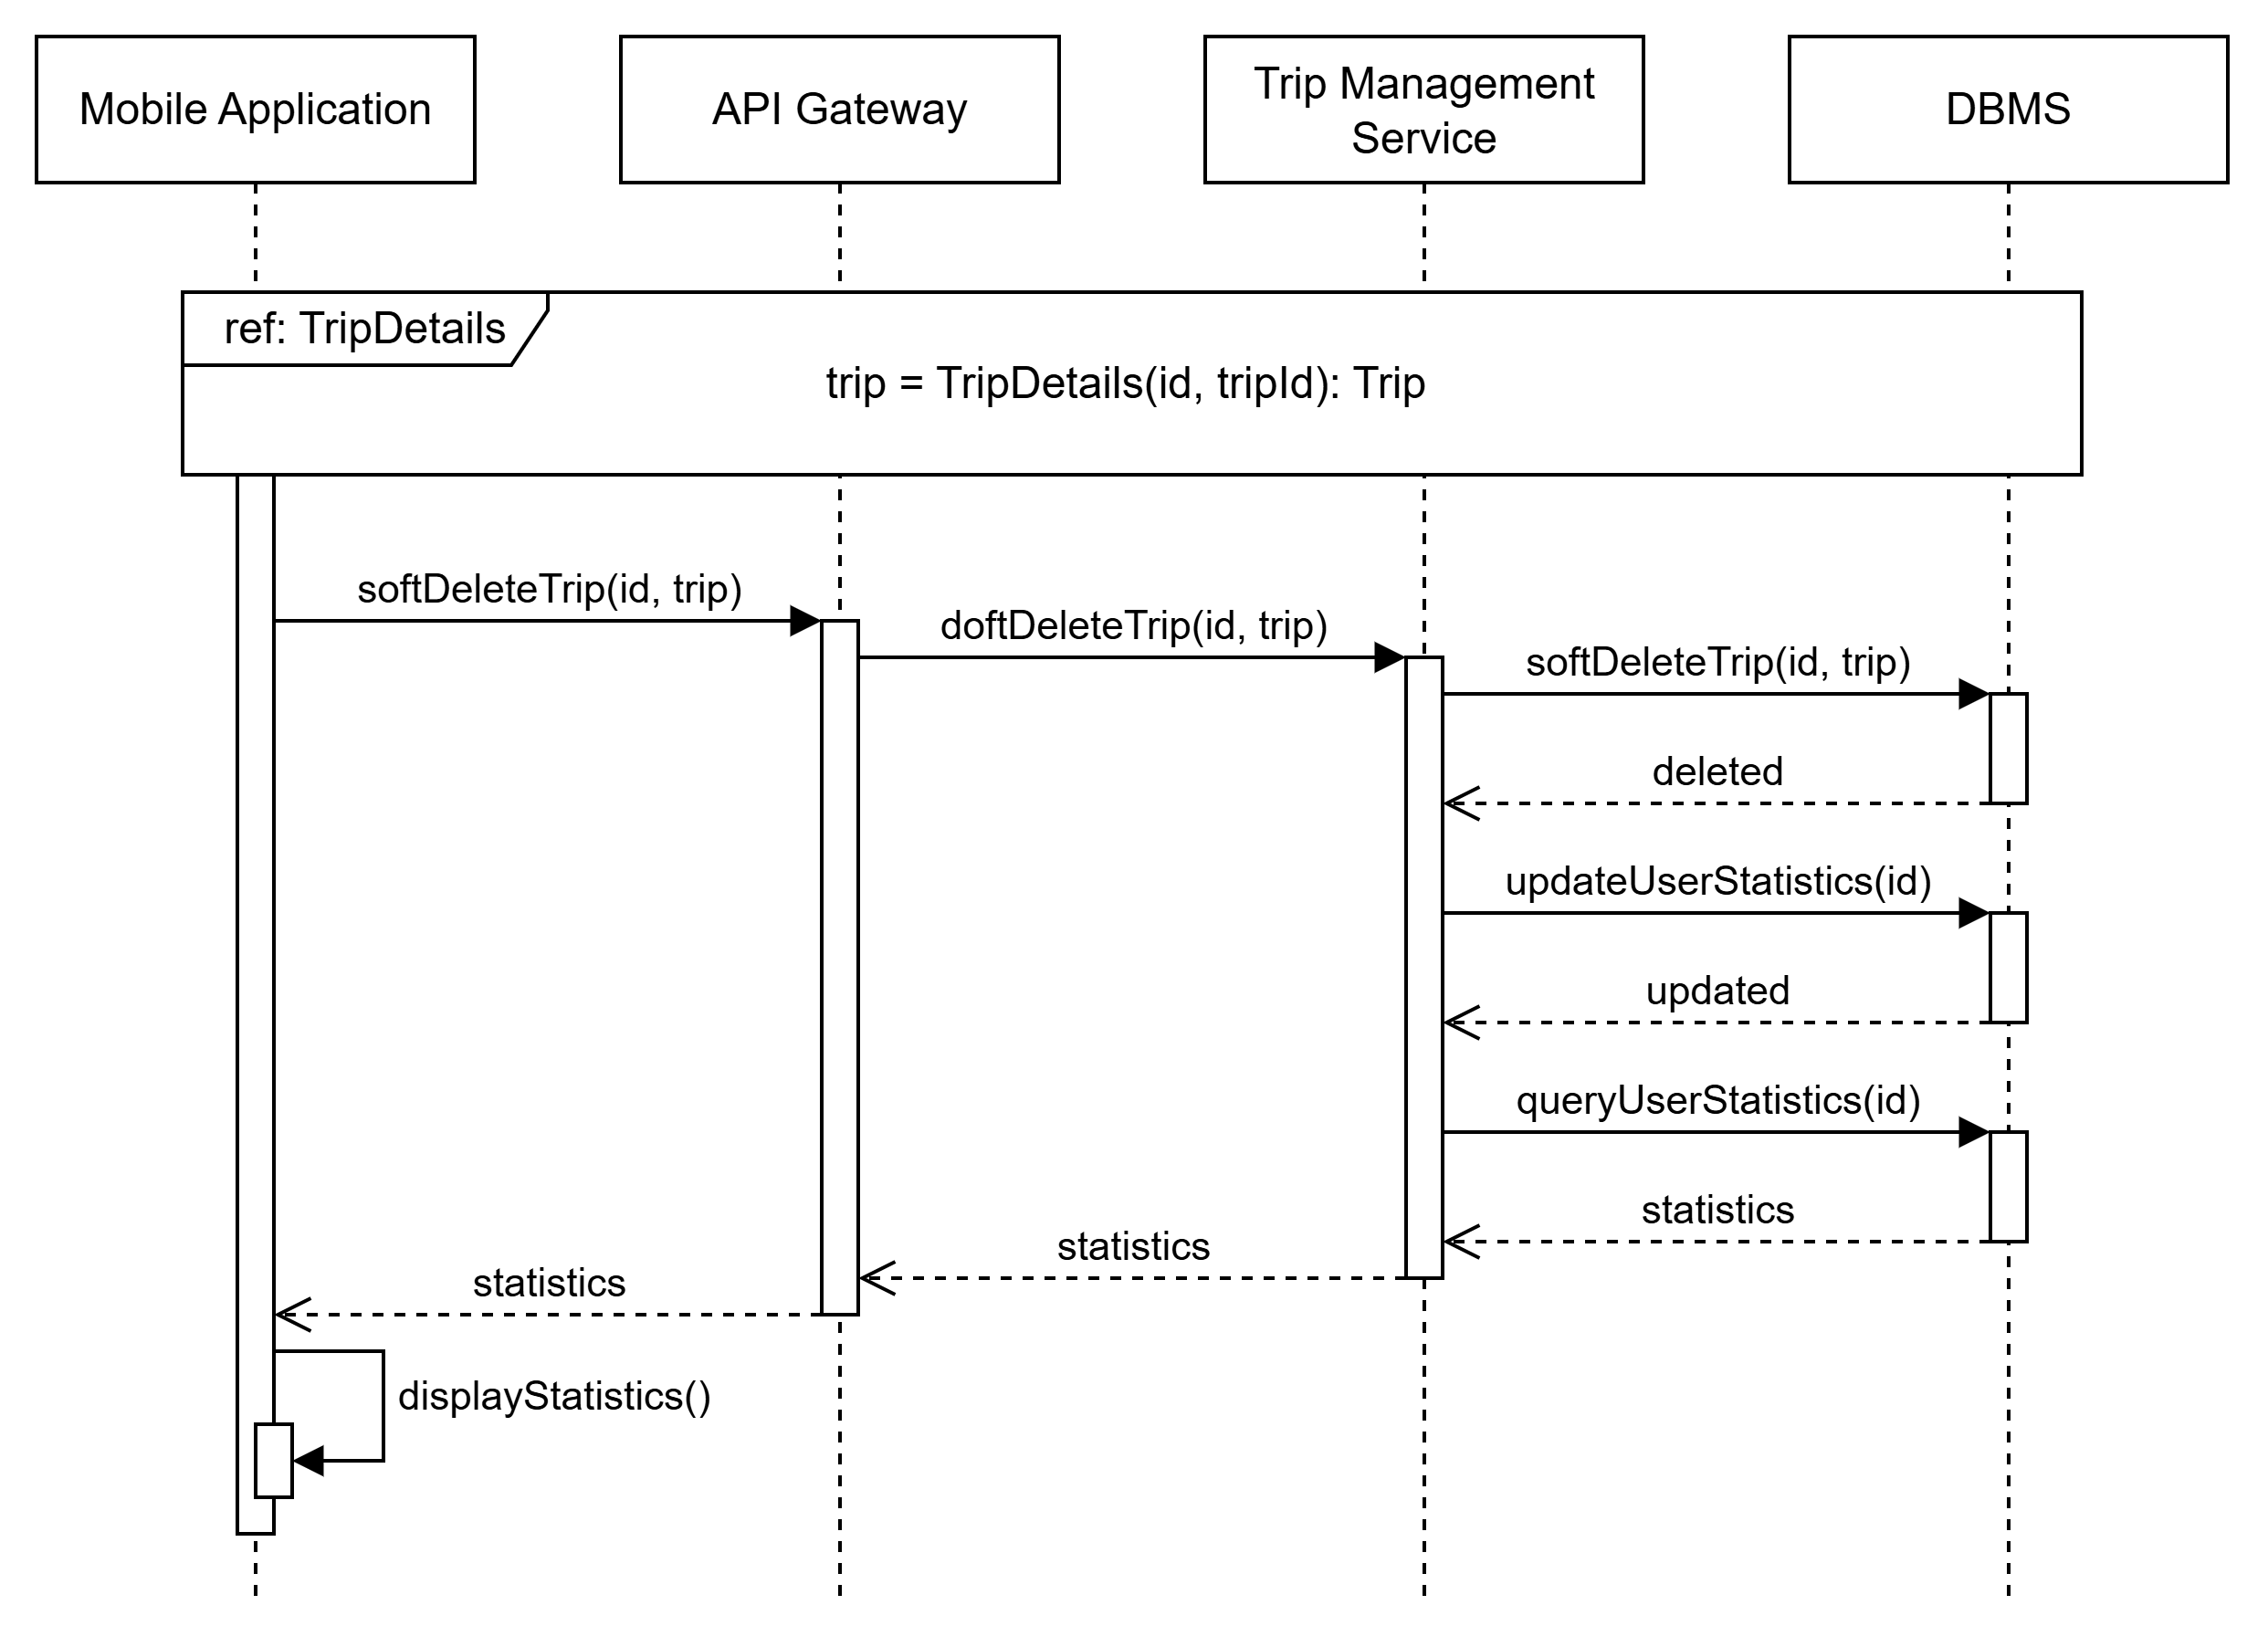
\includegraphics[width=\linewidth]{DD//source//images//diagrams/sd_delete_trip.png}
    \caption{Delete Trips from History Sequence Diagram.}
    \label{fig:delete_trip_sd}
\end{figure}

This sequence diagram shows the interaction between system components during trip deletion. The user can decide to delete a trip after visualizing its details. The client sends a request to the trip management service, which interacts with the DBMS by requesting a soft deletion of the information, the update of user global statistics and the query of the new ones, so the user can visualize them.

\newpage
\noindent
\textbf{UC10: Manual Report}
\begin{figure}[H]
    \centering
    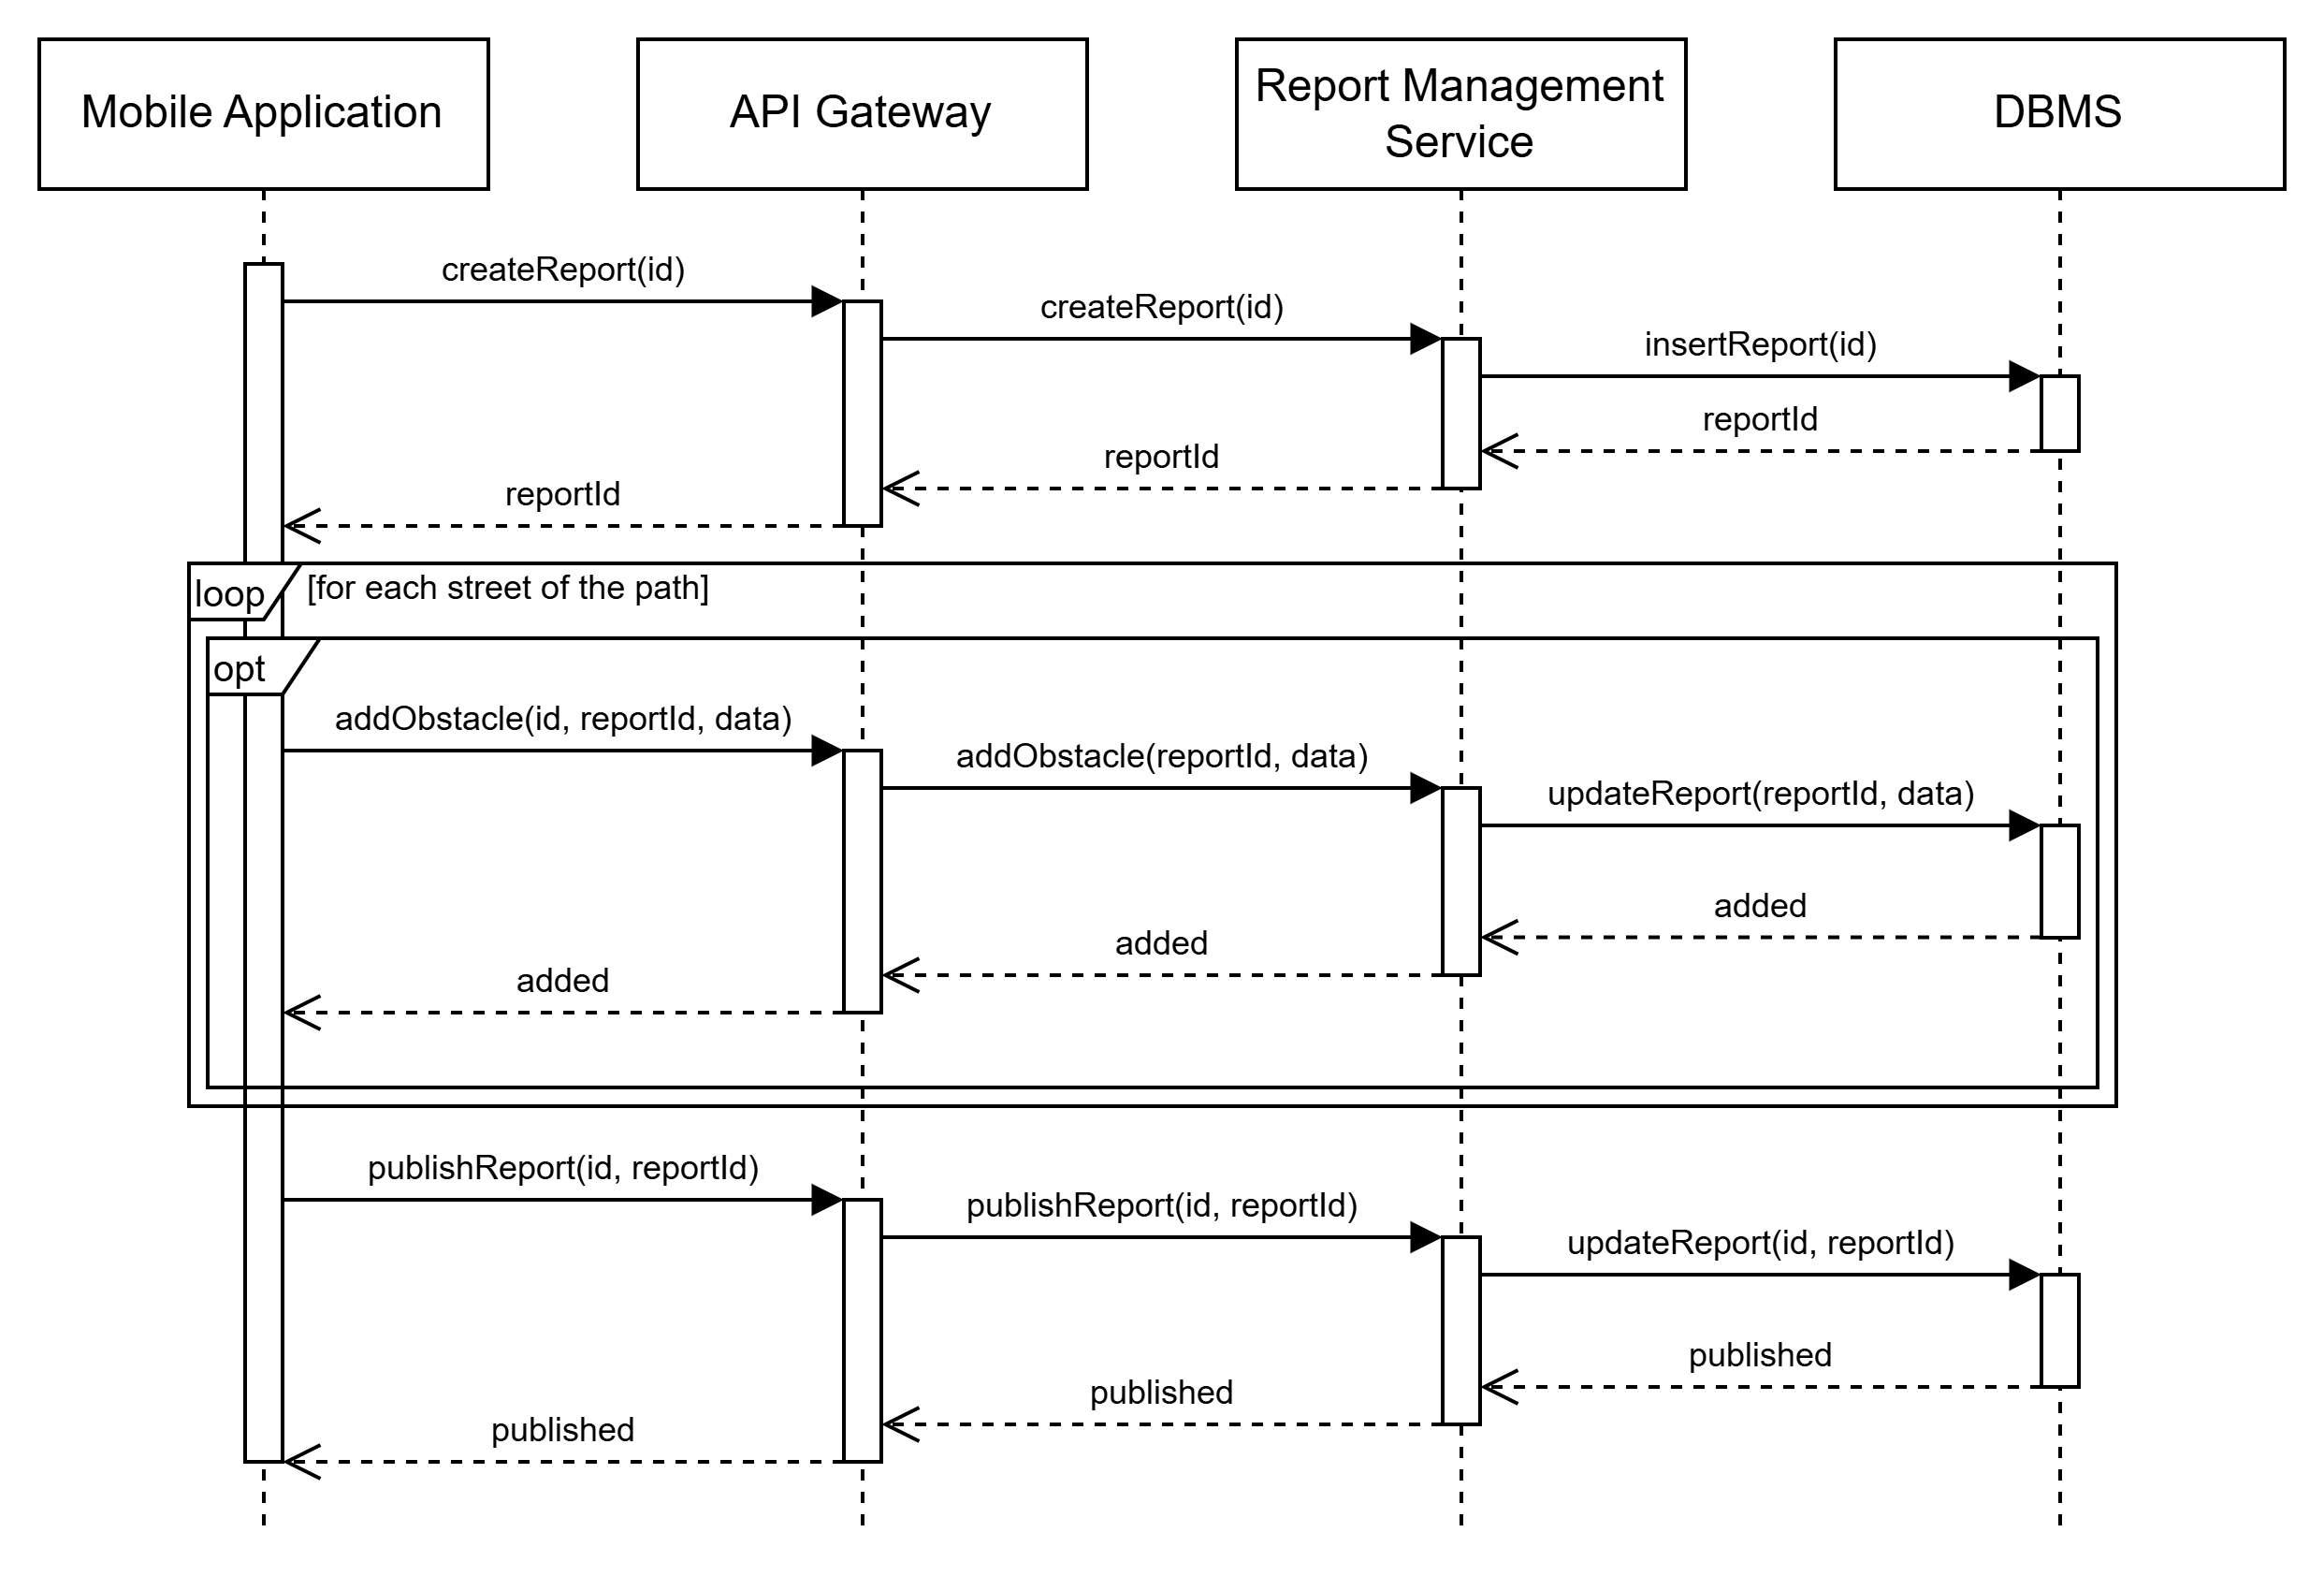
\includegraphics[width=\linewidth]{DD//source//images//diagrams/sd_manual.png}
    \caption{Manual Report Sequence Diagram.}
    \label{fig:manual_sd}
\end{figure}

This sequence diagram shows the interaction between system components during manual reporting. After completing his trip, the user can compile the report regarding the bike path he followed. A creation request is dispatched from the client to the report management system, which creates a new draft and inserts it into the database via the DBMS. For each street of the path, the user can add a new obstacle, which is done once again via a request to the report management service. Once the validation process is completed, the user may optionally publish the data: the client sends a request to the report management component which updates the state of the report, and publishes a new \code{ReportPublished} (\code{RP}) event on the bus, which triggers a synchronization process in the application layer to make the data up-to-date. 

\newpage
\noindent
\textbf{UC11: Automatic Report}
\begin{figure}[H]
    \centering
    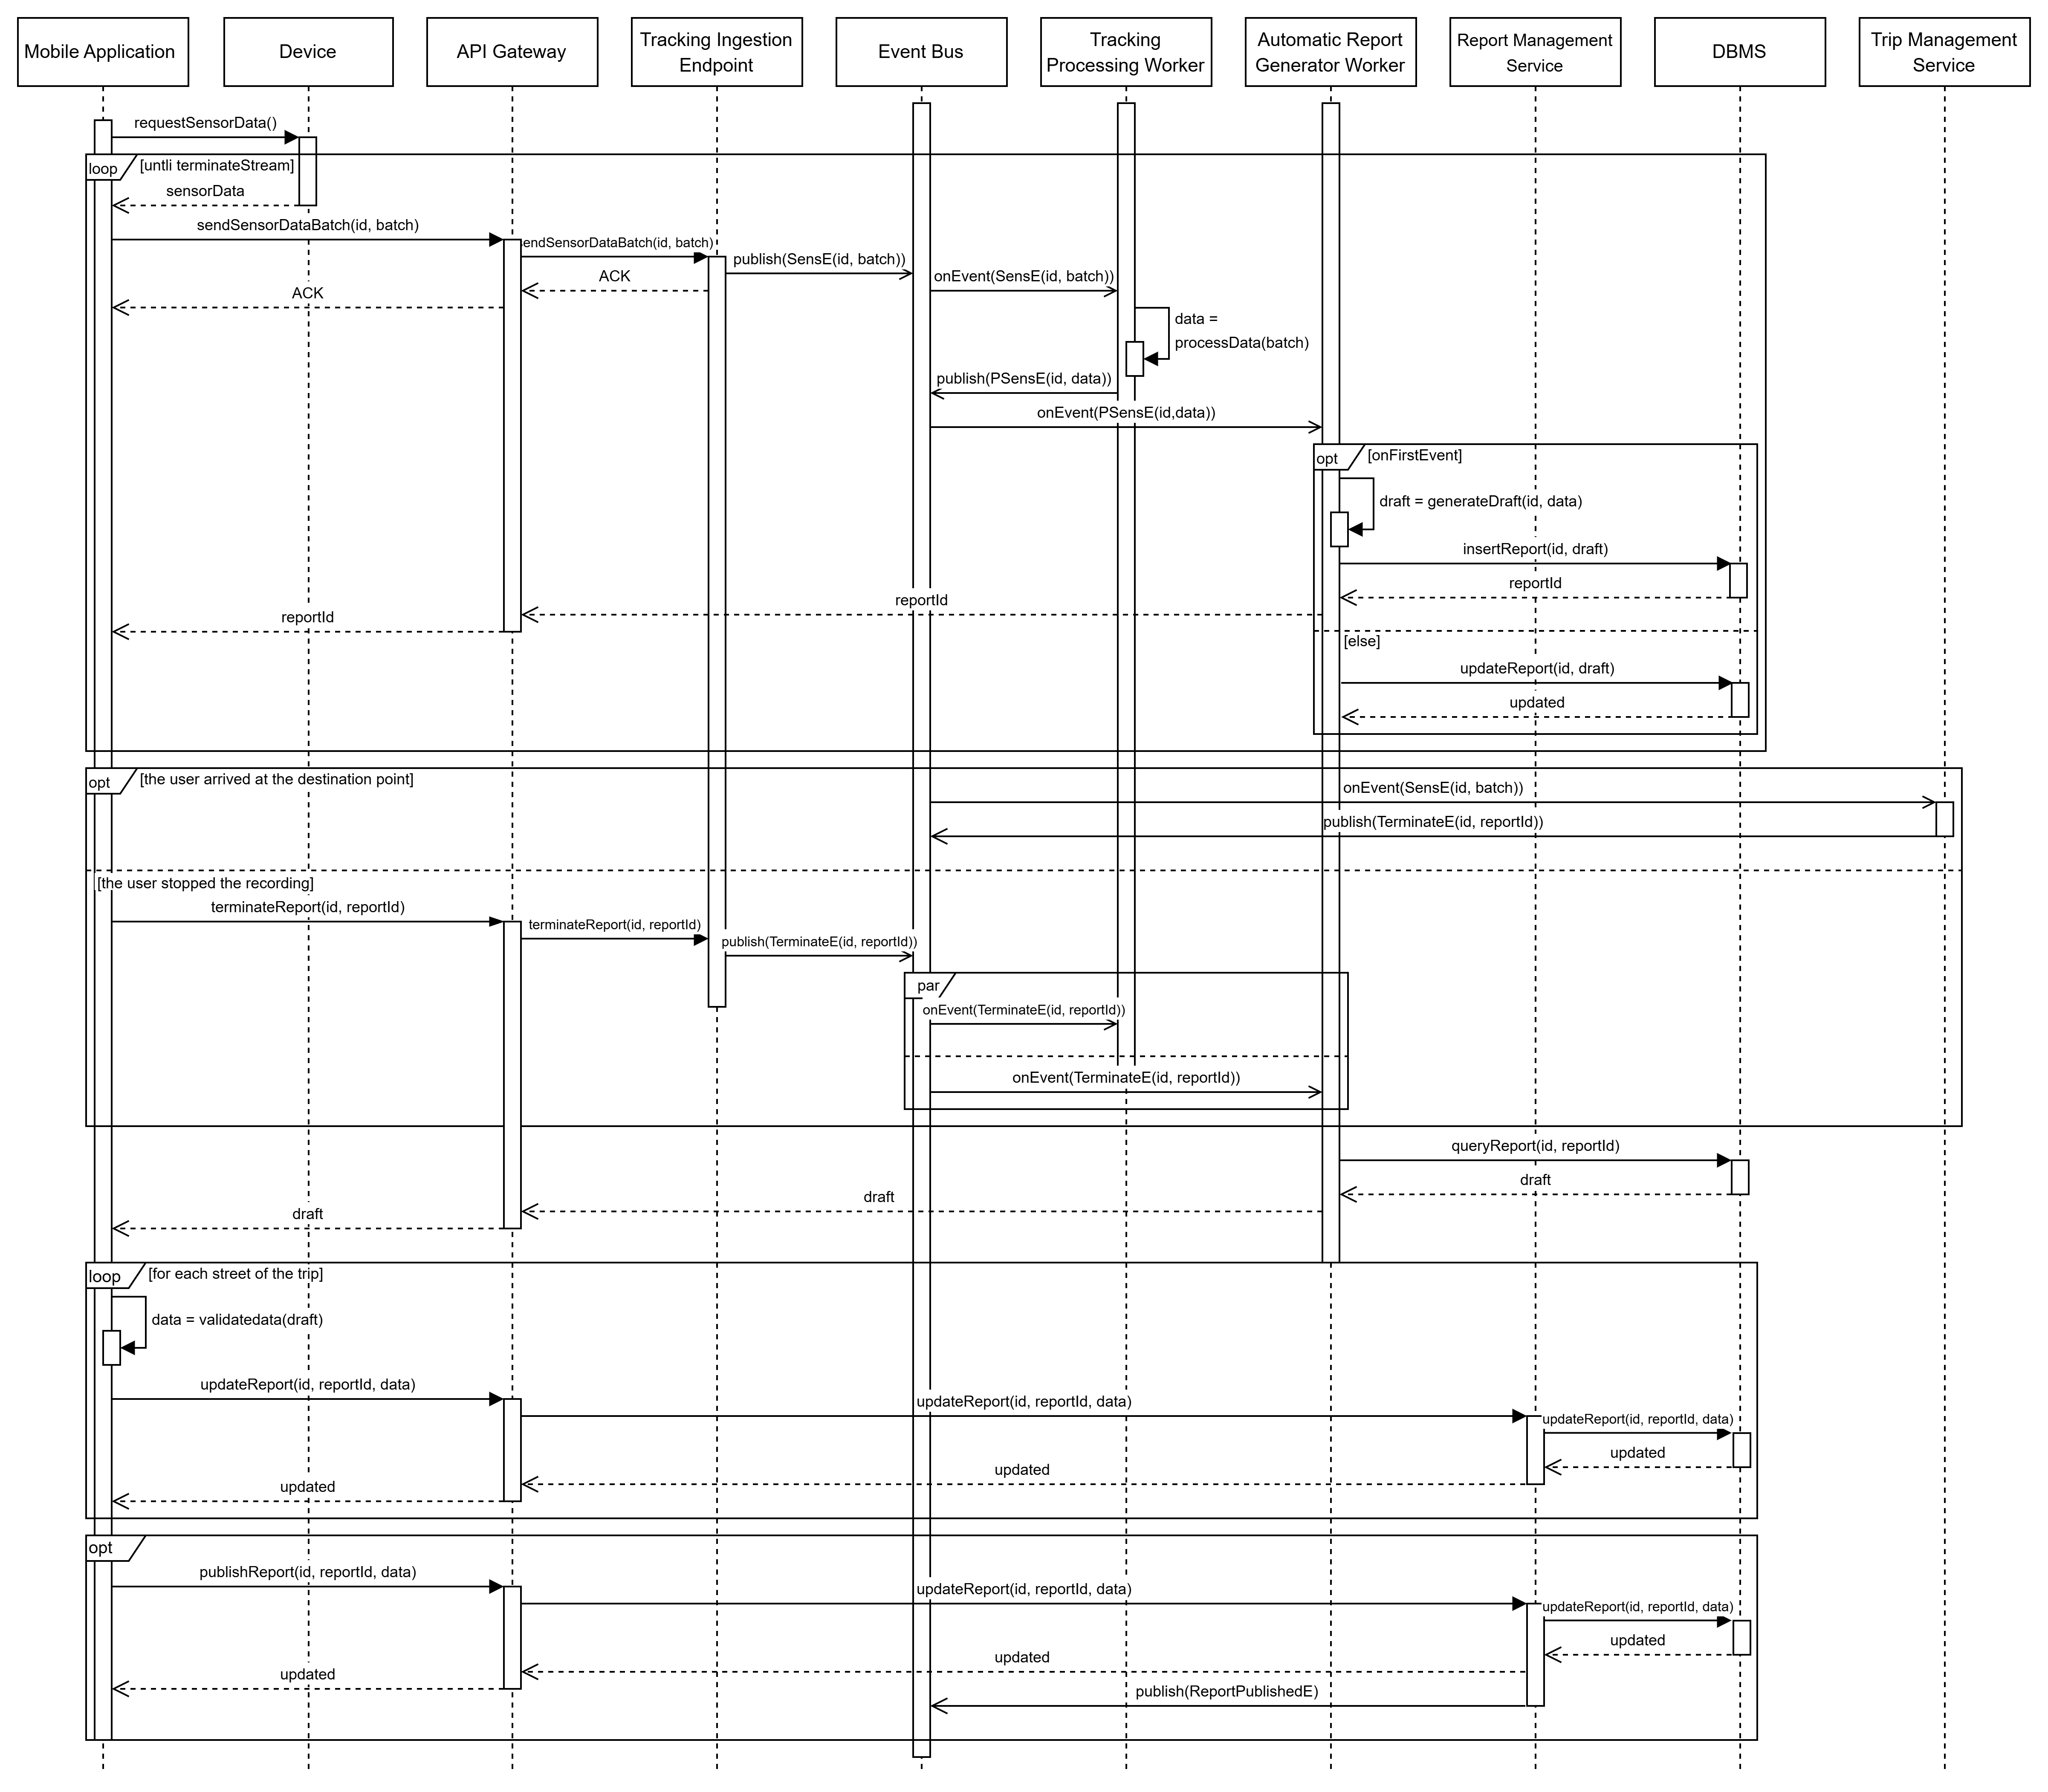
\includegraphics[width=\linewidth]{DD//source//images//diagrams/sd_automatic.png}
    \caption{Automatic Report Sequence Diagram.}
    \label{fig:automatic_sd}
\end{figure}

This sequence diagram shows the interactions between system components during automatic report generation. Once the user starts his trip, the mobile application receives the sensor data, including GPS location, from the device. The client batches all the data and sends it to the tracking ingestion endpoint, which simply publishes to the bus a \code{TrackingDataReceived} (\code{TDR}) event containing the batch. The tracking processing worker reacts to this event by cleaning the data and publishing in turn a new \code{TrackingDataProcessed} (\code{TDP}) event to the bus. This triggers a sequence of tasks in the automatic report generator worker, which creates a new report draft, inserts it into the database, via the DBMS component, and updates it when a new \code{TDP} event is captured from the bus. When the user reaches the destination point, or stops the recording of the trip, a termination event is published into the bus by either the trip management component or the tracking ingestion endpoint respectively. This event is consumed by the automatic report generator, which queries the draft from the DBMS and sends it to the client, so the user can validate the report. Every validation step executed by the user triggers an update to the database, until the verification is completed. At this point the user may optionally publish the data: the client sends a request to the report management component which updates the state of the report, and publishes a new event on the bus, which triggers a synchronization process in the application layer to make the data up-to-date. 

\vspace{0.5cm}
\noindent
\textbf{UC12: Receive Trip Alerts}
\begin{figure}[H]
    \centering
    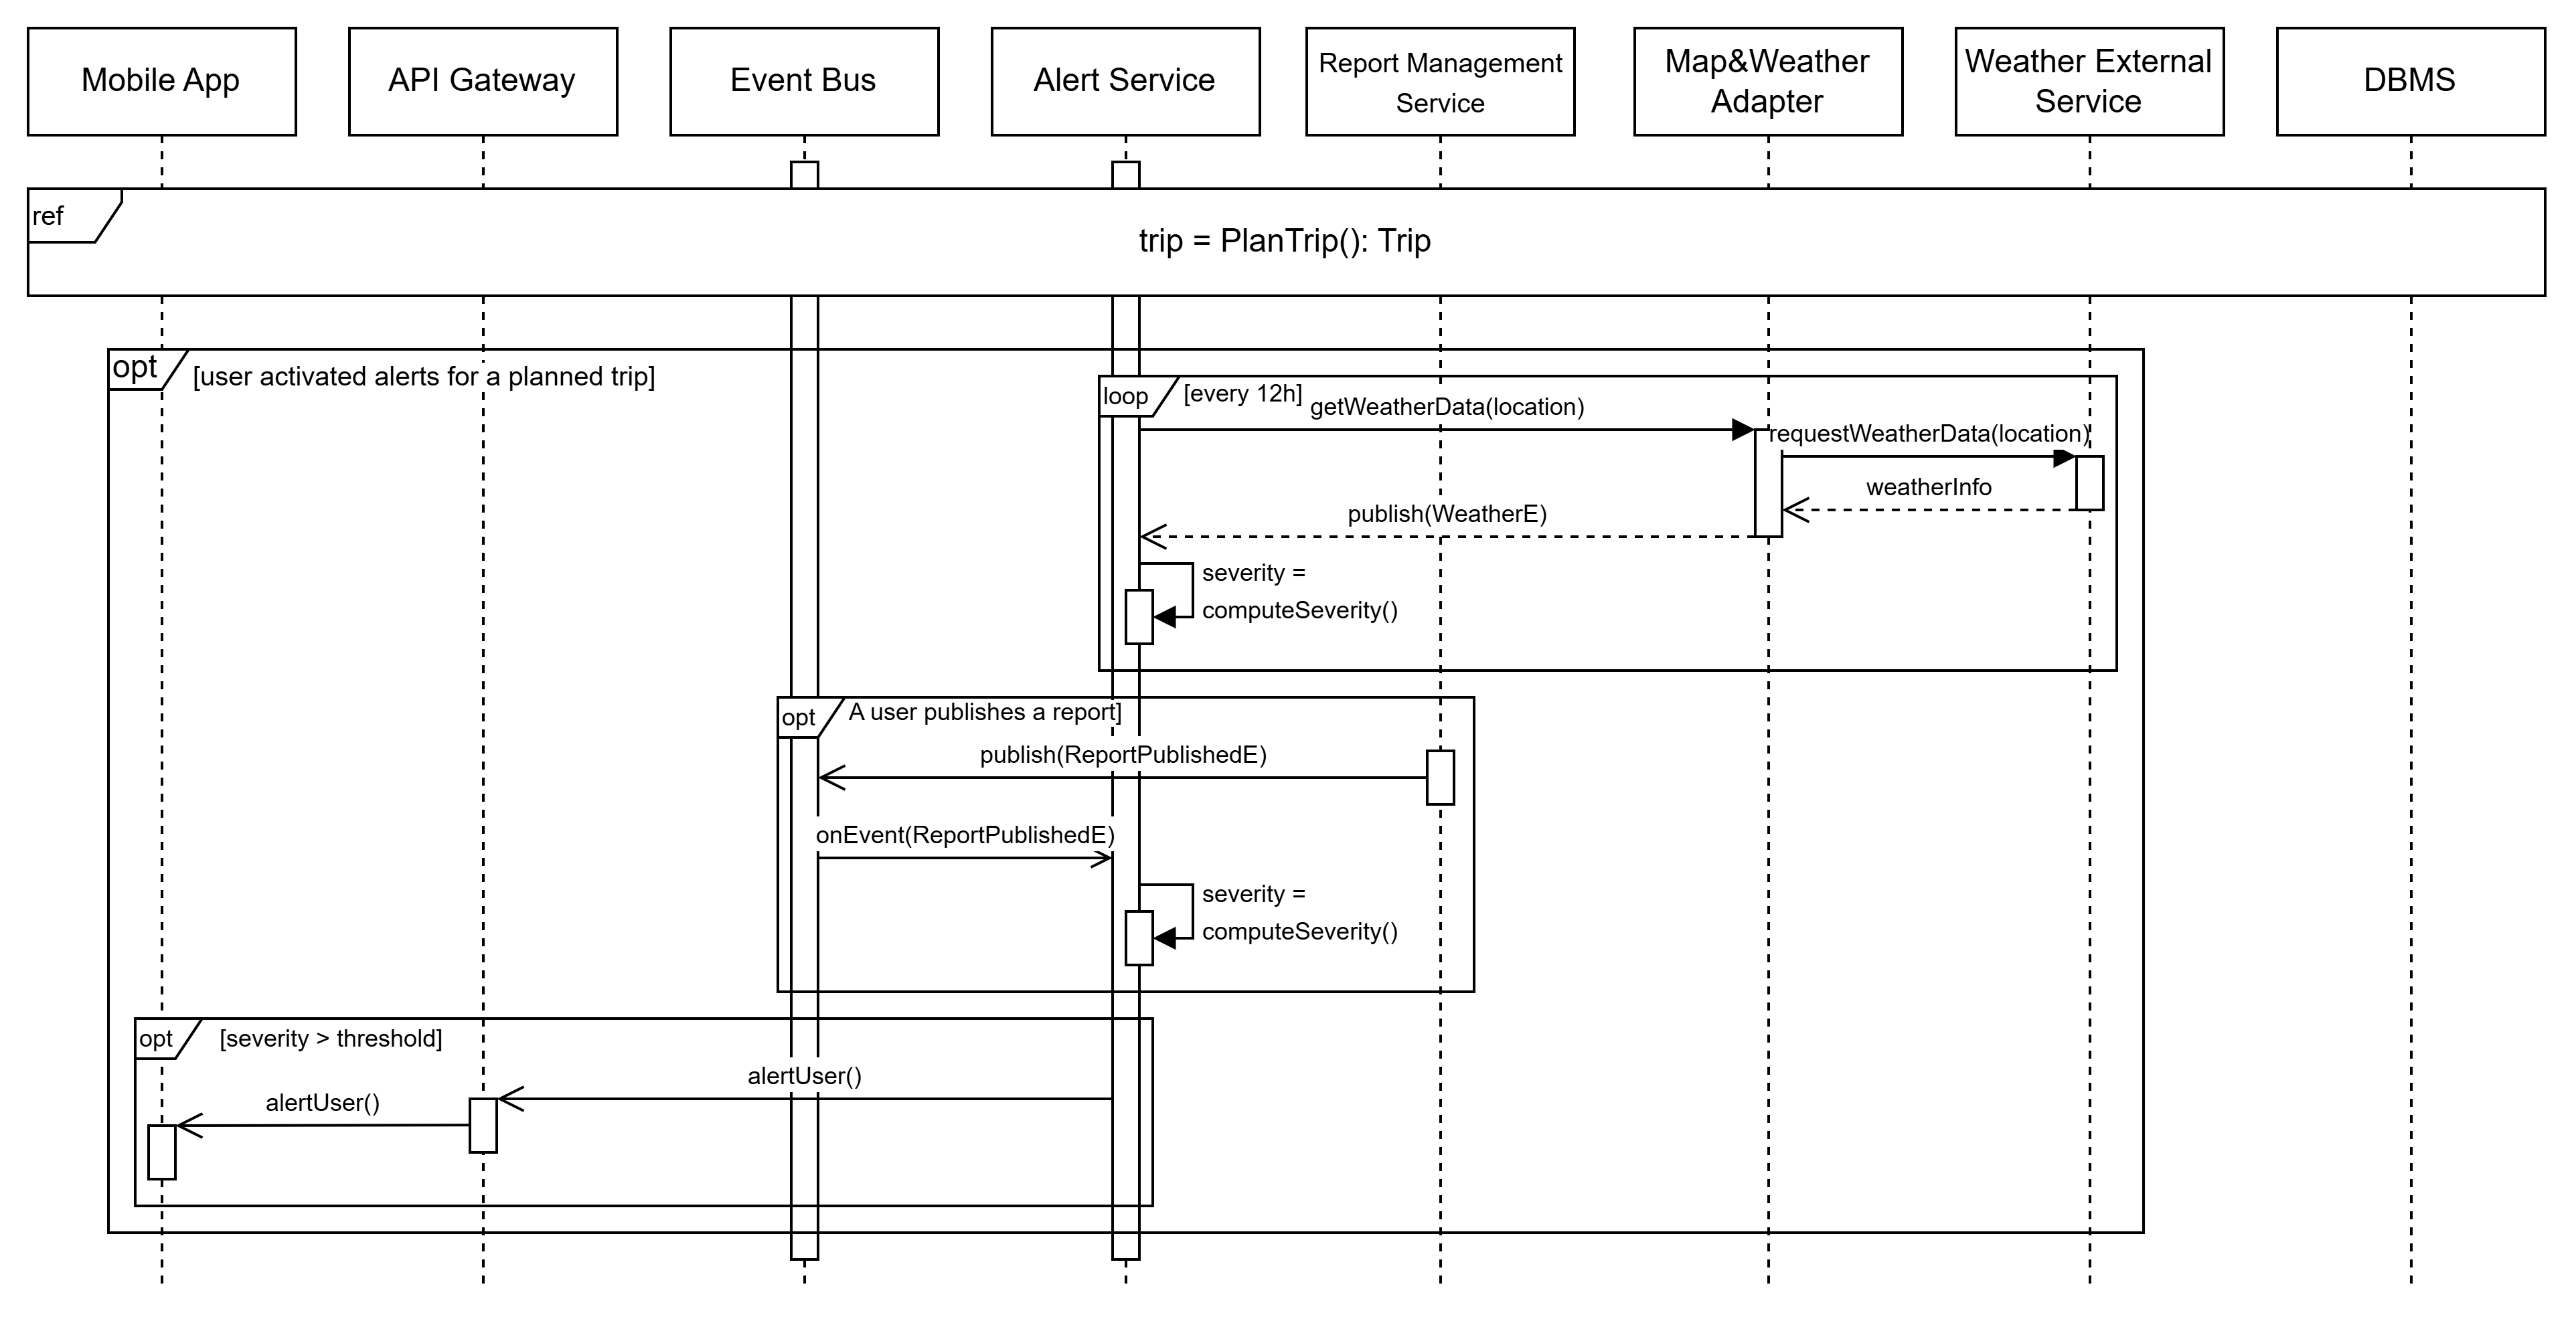
\includegraphics[width=\linewidth]{DD//source//images//diagrams/sd_alerts.png}
    \caption{Receive Trip Alerts Sequence Diagram.}
    \label{fig:alerts_sd}
\end{figure}

This sequence diagram shows the interactions between system components during trip alerts. Once the user has planned a trip, the system activates a polling mechanism that every 12 hours requests weather information to the external weather provider, via the adapter. The alert component, upon receiving the weather data, computes a severity score.  Also, every time the report management service publishes a \code{ReportPublished} (\code{RP}) event on the bus, the alert service reacts by recomputing the severity score. When the score exceeds a given threshold, the alert service triggers a notification to the user's device. 


\subsection{Component Interfaces}
All internal system components interact with each other via gRPC, which is a highly efficient protocol to minimize communication latency. Note that in all previous diagrams the \code{id} passed in almost every function call is the id of the user requesting the represented operations. Technically, the communication between the client and the server is done via the HTTPS protocol, which includes the id in the body, while in internal procedure calls it is necessary to pass it as argument to perform the requested operations.

\newpage
\paragraph{API}
\begin{itemize}
    \item register(name, surname, email, hashedPassword)
    \item login(email, hashedPassword)
    \item deleteAccount(id)
    \item getMapData(id, location)
    \item getWeatherData(id, location)
    \item getPathsBy(id, departure, destination, filter)
    \item getPathsInArea(id, location, filter)
    \item getPathDetails(id, pathId)
    \item saveTrip(id, pathId)
    \item switchPreferences(id, preferences)
    \item getGlobalStatistics(id)
    \item getPlannedTrips(id)
    \item getCompletedTrips(id)
    \item getTripInfo(id, tripId)
    \item deletePlannedTrip(id, tripId)
    \item createReport(id)
    \item addObstacle(id, reportId, data)
    \item publishReport(id, reportId)
    \item sendSensorDataBatch(id, data)
    \item terminateAutomaticReport(id, reportId)
    \item updateAutomaticReport(id, reportId, data)
\end{itemize}

\paragraph{User Management Service Interface}
\begin{itemize}
    \item registerUser(name, surname, email, hashedPassword)
    \item logIn(email, hashedPassword)
    \item updateProfile(id, data)
    \item deleteAccount(id)
\end{itemize}

\paragraph{Path Exploration Service Interface}
\begin{itemize}
    \item getPaths(departure, destination, filter)
    \item getPaths(location, filter)
    \item getPathDetails(pathId)
\end{itemize}

\paragraph{Trip Management Service Interface}
\begin{itemize}
    \item saveTrip(id, pathId)
    \item getGlobalStatistics(id)
    \item getPlannedTrips(id)
    \item getCompletedTrips(id)
    \item getTripInfo(tripId)
    \item deletePlannedtrip(id, tripId)
\end{itemize}

\paragraph{Report Management Service Interface}
\begin{itemize}
    \item createReport(id)
    \item addObstacle(id, reportId, data)
    \item deleteObstacle(id, reportId, data)
    \item publishReport(id, reportId, data)
    \item updateReport(id, reportId, data)
\end{itemize}

\paragraph{Map \& Weather Adapter Interface}
\begin{itemize}
    \item getMapData(location)
    \item getWeatherData(location)
\end{itemize}

\paragraph{Event Bus Interface}
\begin{itemize}
    \item subscribe()
    \item publish(Event)
\end{itemize}

\paragraph{Tracking Ingestion Endpoint Interface}
\begin{itemize}
    \item sendSensorDataBatch(id, data)
\end{itemize}

\paragraph{Tracking Processing Worker Interface}
The tracking processing worker component only reacts to \code{SensE(id, batch)} events on the bus, so it does not have an interface, other than the one needed for the publish-subscribe pattern.

\paragraph{Automatic Report Generator Worker Interface}
The automatic report generator worker component only reacts to \code{PSensE(id, data)} events on the bus, so it does not have an interface, other than the one needed for the publish-subscribe pattern.

\paragraph{Alert Service Worker Interface}
\begin{itemize}
    \item alertUser()
\end{itemize}

\paragraph{Database Management System Interface}
\begin{itemize}
    \item insertUser(name, surname, email, hashedPassword)
    \item queryUser(email, hashedPassword)
    \item updateUser(id, data)
    \item deleteUser(id)
    \item queryPaths(departure, destination, filter)
    \item querypaths(location, filter)
    \item queryPathDetails(pathId)
    \item insertPlannedTrip(id, pathId)
    \item updatePreferences(id, preferences)
    \item queryUserStatistics(id)
    \item queryPlannedTrips(id)
    \item queryCompletedTrips(id)
    \item queryTripDetails(tripId)
    \item softDeleteTrip(id, tripId)
    \item updateUserStatistics(id)
    \item insertReport(id, draft)
    \item updateReport(id, reportId, data)
    \item queryReport(id, reportId)
\end{itemize}

\subsection{Selected Architectural Styles and Patterns}
\paragraph{3 Tier Architecture}
The BBP system is designed upon a robust three-tier client-server architecture, enhanced by an event driven layer. This design decouples the interactions the user has with the platform from the services it provides, without slowing down the user experience, as heavy computational tasks can be processed in the background avoiding latency. The resulting loose coupling brings great flexibility and facilitates horizontal scalability of the back-end as components can be deployed as micro-services, which can be replicated across distributed servers to accommodate for the growing user demand. Also, it guarantees grater security, as every component of the application layer is developed to comply with the GDPR regulations and best security practices.

\paragraph{Event-Driven Architecture}
Most of the interactions between the client and the server, but also between the components of the application layer, are synchronous, but there are some critical features that require a more complex architecture: hence the need to add an asynchronous event driven layer, which allows some heavy computational tasks to be processed in the background without interrupting the user experience flow. More specifically, this hybrid architecture features an event bus component which streams a queue of messages other components of the system can listen and react to. This allows low latency components to communicate with heavy duty ones, without the need of complex synchronization between them.

\paragraph{Microservice Architecture}
As already mentioned, the microservice architecture design best fits the need of a resilient and scalable system to allow the user to interact with the feature-rich BBP platform. The presentation layer communicates with the components the application layer is made of via the API gateway, which constitutes the entry point of the back-end service, allowing the client an easy and controlled access to the platform. Microservices communicate with each other via a high efficiency protocol, like gRPC, allowing faster data retrieval and a more structured and robust system, without compromising flexibility. Also, the microservice architecture allows the deployment of the components across a distributed system, so it is easier to horizontally scale up the back-end to accommodate for growing user demand.

\paragraph{Circuit Breakers}
The system requires to be highly available to the end users of the platform, to ensure uninterrupted service at all times. To achieve this objective, the circuit breaker pattern is integrated within the application layer to prevent cascading failures, effectively isolating faults when service latency or failures are detected.

\paragraph{State Pattern}
The central core of the system is obstacle information, which is gathered by means of reports compiled by users. Careful management of this data is therefore crucial to ensure the system functions correctly. To achieve this objective, the management of the reports is implemented using the state pattern, which also minimizes data loss.

\paragraph{Publish Subscribe Pattern}
As already mentioned in previous sections, the asynchronous nature of some features of the platform led 
to the adoption of an hybrid architecture with an Event-Driven layer, implemented using a publish-subscribe pattern. More specifically, asynchronous components subscribe to the event bus, listening to the stream of events and reacting to those that concern them. This design decision prevents tight coupling of components and makes asynchronous tasks effortless.

\paragraph{Adapter}
Some features of the platform rely on external services, such as map and weather solutions, to enrich the user experience. The adapter pattern becomes a necessity as data from external services have a different structure from that used by the system. Some components of the application layer, namely the Map and Weather Adapter, act as a link between the external and the internal services, providing an interface through which the platform is able to communicate. It also allows timeout handling, fallback strategies, and graceful degradation in case of service unavailability. 

